% Options for packages loaded elsewhere
\PassOptionsToPackage{unicode}{hyperref}
\PassOptionsToPackage{hyphens}{url}
%
\documentclass[
  english,
  man,floatsintext]{apa6}
\usepackage{amsmath,amssymb}
\usepackage{lmodern}
\usepackage{ifxetex,ifluatex}
\ifnum 0\ifxetex 1\fi\ifluatex 1\fi=0 % if pdftex
  \usepackage[T1]{fontenc}
  \usepackage[utf8]{inputenc}
  \usepackage{textcomp} % provide euro and other symbols
\else % if luatex or xetex
  \usepackage{unicode-math}
  \defaultfontfeatures{Scale=MatchLowercase}
  \defaultfontfeatures[\rmfamily]{Ligatures=TeX,Scale=1}
\fi
% Use upquote if available, for straight quotes in verbatim environments
\IfFileExists{upquote.sty}{\usepackage{upquote}}{}
\IfFileExists{microtype.sty}{% use microtype if available
  \usepackage[]{microtype}
  \UseMicrotypeSet[protrusion]{basicmath} % disable protrusion for tt fonts
}{}
\makeatletter
\@ifundefined{KOMAClassName}{% if non-KOMA class
  \IfFileExists{parskip.sty}{%
    \usepackage{parskip}
  }{% else
    \setlength{\parindent}{0pt}
    \setlength{\parskip}{6pt plus 2pt minus 1pt}}
}{% if KOMA class
  \KOMAoptions{parskip=half}}
\makeatother
\usepackage{xcolor}
\IfFileExists{xurl.sty}{\usepackage{xurl}}{} % add URL line breaks if available
\IfFileExists{bookmark.sty}{\usepackage{bookmark}}{\usepackage{hyperref}}
\hypersetup{
  pdftitle={The Development of English Negative Constructions and Communicative Functions in Early Child Language},
  pdfauthor={Zoey Liu1 \& Masoud Jasbi2},
  pdflang={en-EN},
  pdfkeywords={negation; syntactic construction; communicative function; data-driven; child language development.},
  hidelinks,
  pdfcreator={LaTeX via pandoc}}
\urlstyle{same} % disable monospaced font for URLs
\usepackage{longtable,booktabs,array}
\usepackage{calc} % for calculating minipage widths
% Correct order of tables after \paragraph or \subparagraph
\usepackage{etoolbox}
\makeatletter
\patchcmd\longtable{\par}{\if@noskipsec\mbox{}\fi\par}{}{}
\makeatother
% Allow footnotes in longtable head/foot
\IfFileExists{footnotehyper.sty}{\usepackage{footnotehyper}}{\usepackage{footnote}}
\makesavenoteenv{longtable}
\usepackage{graphicx}
\makeatletter
\def\maxwidth{\ifdim\Gin@nat@width>\linewidth\linewidth\else\Gin@nat@width\fi}
\def\maxheight{\ifdim\Gin@nat@height>\textheight\textheight\else\Gin@nat@height\fi}
\makeatother
% Scale images if necessary, so that they will not overflow the page
% margins by default, and it is still possible to overwrite the defaults
% using explicit options in \includegraphics[width, height, ...]{}
\setkeys{Gin}{width=\maxwidth,height=\maxheight,keepaspectratio}
% Set default figure placement to htbp
\makeatletter
\def\fps@figure{htbp}
\makeatother
\setlength{\emergencystretch}{3em} % prevent overfull lines
\providecommand{\tightlist}{%
  \setlength{\itemsep}{0pt}\setlength{\parskip}{0pt}}
\setcounter{secnumdepth}{-\maxdimen} % remove section numbering
% Make \paragraph and \subparagraph free-standing
\ifx\paragraph\undefined\else
  \let\oldparagraph\paragraph
  \renewcommand{\paragraph}[1]{\oldparagraph{#1}\mbox{}}
\fi
\ifx\subparagraph\undefined\else
  \let\oldsubparagraph\subparagraph
  \renewcommand{\subparagraph}[1]{\oldsubparagraph{#1}\mbox{}}
\fi
% Manuscript styling
\usepackage{upgreek}
\captionsetup{font=singlespacing,justification=justified}

% Table formatting
\usepackage{longtable}
\usepackage{lscape}
% \usepackage[counterclockwise]{rotating}   % Landscape page setup for large tables
\usepackage{multirow}		% Table styling
\usepackage{tabularx}		% Control Column width
\usepackage[flushleft]{threeparttable}	% Allows for three part tables with a specified notes section
\usepackage{threeparttablex}            % Lets threeparttable work with longtable

% Create new environments so endfloat can handle them
% \newenvironment{ltable}
%   {\begin{landscape}\centering\begin{threeparttable}}
%   {\end{threeparttable}\end{landscape}}
\newenvironment{lltable}{\begin{landscape}\centering\begin{ThreePartTable}}{\end{ThreePartTable}\end{landscape}}

% Enables adjusting longtable caption width to table width
% Solution found at http://golatex.de/longtable-mit-caption-so-breit-wie-die-tabelle-t15767.html
\makeatletter
\newcommand\LastLTentrywidth{1em}
\newlength\longtablewidth
\setlength{\longtablewidth}{1in}
\newcommand{\getlongtablewidth}{\begingroup \ifcsname LT@\roman{LT@tables}\endcsname \global\longtablewidth=0pt \renewcommand{\LT@entry}[2]{\global\advance\longtablewidth by ##2\relax\gdef\LastLTentrywidth{##2}}\@nameuse{LT@\roman{LT@tables}} \fi \endgroup}

% \setlength{\parindent}{0.5in}
% \setlength{\parskip}{0pt plus 0pt minus 0pt}

% \usepackage{etoolbox}
\makeatletter
\patchcmd{\HyOrg@maketitle}
  {\section{\normalfont\normalsize\abstractname}}
  {\section*{\normalfont\normalsize\abstractname}}
  {}{\typeout{Failed to patch abstract.}}
\patchcmd{\HyOrg@maketitle}
  {\section{\protect\normalfont{\@title}}}
  {\section*{\protect\normalfont{\@title}}}
  {}{\typeout{Failed to patch title.}}
\makeatother
\shorttitle{Children's Negative Constructions and Communicative Functions}
\keywords{negation; syntactic construction; communicative function; data-driven; child language development.
\newline\indent Word count: X}
\usepackage{lineno}

\linenumbers
\usepackage{csquotes}
\ifxetex
  % Load polyglossia as late as possible: uses bidi with RTL langages (e.g. Hebrew, Arabic)
  \usepackage{polyglossia}
  \setmainlanguage[]{english}
\else
  \usepackage[main=english]{babel}
% get rid of language-specific shorthands (see #6817):
\let\LanguageShortHands\languageshorthands
\def\languageshorthands#1{}
\fi
\ifluatex
  \usepackage{selnolig}  % disable illegal ligatures
\fi
\newlength{\cslhangindent}
\setlength{\cslhangindent}{1.5em}
\newlength{\csllabelwidth}
\setlength{\csllabelwidth}{3em}
\newenvironment{CSLReferences}[2] % #1 hanging-ident, #2 entry spacing
 {% don't indent paragraphs
  \setlength{\parindent}{0pt}
  % turn on hanging indent if param 1 is 1
  \ifodd #1 \everypar{\setlength{\hangindent}{\cslhangindent}}\ignorespaces\fi
  % set entry spacing
  \ifnum #2 > 0
  \setlength{\parskip}{#2\baselineskip}
  \fi
 }%
 {}
\usepackage{calc}
\newcommand{\CSLBlock}[1]{#1\hfill\break}
\newcommand{\CSLLeftMargin}[1]{\parbox[t]{\csllabelwidth}{#1}}
\newcommand{\CSLRightInline}[1]{\parbox[t]{\linewidth - \csllabelwidth}{#1}\break}
\newcommand{\CSLIndent}[1]{\hspace{\cslhangindent}#1}

\title{The Development of English Negative Constructions and Communicative Functions in Early Child Language}
\author{Zoey Liu\textsuperscript{1} \& Masoud Jasbi\textsuperscript{2}}
\date{}


\authornote{

Zoey Liu, Department of Computer Science, Boston College
Masound Jasbi, Department of Linguistics, University of California, Davis

Correspondence concerning this article should be addressed to Zoey Liu, . E-mail: \href{mailto:zoey.liu@bc.edu}{\nolinkurl{zoey.liu@bc.edu}}

}

\affiliation{\vspace{0.5cm}\textsuperscript{1} Boston College\\\textsuperscript{2} Uinversity of California, Davis}

\abstract{
How does the abstract concept of linguistic negation develop in early child language? Prior research has suggested that the concept of negation develops from more concrete communicative functions such as rejection, prohibition, or non-existence, with each function emerging in different stages. The evidence for the emergence of these functions in separate stages is mixed, however, leaving the possibility that negation is an abstract concept that can serve multiple specific functions since the beginning, and that the development of the different functions start more or less simutanouesly depending on early communicative environment. Leveraging automatic annotations of large-scale child speech corpora in English, we examine the production trajectores of seven negative constructions that tend to convey communicative functions previously discussed in the literature. The results demonstrate the emergence and gradual increase of these constructions in child speech within the age range of 18-36 months at both sentence and discourse level. Production mostly becomes stable, regular, and comparable to parents' levels after this age range. These findings suggest that different communicative functions of negation share comparable production trajectory and do not clearly follow a fixed developmental order. Alternatively, it is possible that these functions emerge so early and quickly that even though they might develop in different stages, it is not detectable from the available corpus data.
}



\begin{document}
\maketitle

\hypertarget{introduction}{%
\section{Introduction}\label{introduction}}

Negation is a basic human concept and foundational to many areas of human thought including logic and mathematics (Haspelmath, 1997; Jespersen, 1917). An important feature of linguistic negation is that it has an abstract meaning and serves different communicative functions in different contexts. In English, for example, a coffee shop can use \emph{not} to divide the menu into ``coffee'' and ``not coffee'' sections, with ``not coffee'' bringing together diverse items such as tea and hot chocolate. The coffee shop can use \emph{no} in a sign like ``no mask, no entry'' to regulate customer behavior, and an employee could say ``I don't like Mondays'' to express their dislike for coming back to work on Mondays. Despite its abstract meaning, a word like \emph{no} is among the early words produced by children. Therefore, a fundamental question in cognitive development and language acquisition is how negation emerges and develops in the human mind. Is early development of negation in child language specific to a few communicative functions? Or does negation emerge as an abstract and multi-functional concept from the beginning?

Previous literature has proposed that abstract negation develops from less abstract communicative functions in a fixed order (Bloom, 1970; Choi, 1988; McNeill \& McNeill, 1968; Pea, 1978). In other words, different functions of negation have been argued to have separate \emph{stages} of acquisition. For instance, Darwin (1872) hypothesized that headshake as a sign for negation develops from infants' habit to refuse or reject food from parents by withdrawing their heads. Similarly, Pea (1978) proposed that at first, children use \emph{no} to convey ``rejection.'' In a second stage, they conceptualize and express non-existence of objects (e.g., ``no water {[}in the cup{]}''), and finally in the third stage, negation reaches an abstract status that can deny truth of statements (e.g., ``that is not a cow''). For Pea (1978), this order reflected a natural progression in the conceptual space: from the more primitive domain of internal desires to the more complex domain of external existence, and finally abstract truth.

As we will discuss in the next section, as fruitful as prior work is, their theoretical and empirical landscape is not always so clean. Therefore while negation does serve multiple communicative functions, there has been no consensus reached regarding two respects:

\begin{enumerate}
\def\labelenumi{(\arabic{enumi})}
\item
  Does negation develop from different communicative functions in fixed ordered stages?
\item
  If so, what is the developmental order of these functions?
\end{enumerate}

In this study, we take up the aforementioned two questions with a data-driven approach. Leveraging child-speech corpora in English, we investigate the developmental patterns of seven communicative functions of negation that have gained much attention in prior research. On the basis that children's early linguistic production reflects developmental stages, our results suggest that negation starts as an abstract concept that can be used to perform multiple communicative functions from the beginning, depending on the demands of early linguistic interactions. The overall developmental trajectory of each funciton is similar to each other in terms of when the production of the funciton emerges, the estimated maximum capacity of production, and the point at which production starts to become stable. This findings do not seem to provide clear evidence for what has been widely speculated in the literature, which posits that the developmental paths of separate communicative functions of negation are noticeably different. In what follows, we review previous studies on children's production of negation, then move on to details of our own experiments.

\hypertarget{previous-studies}{%
\section{Previous Studies}\label{previous-studies}}

Darwin (1872, Chapter 11) explained the emergence of linguistic negation using the function it plays in early communication. He hypothesized that nodding and shaking are the earliest expressions of affirmation and negation respectively and argued:

With infants, the first act of denial consists in refusing food; and I repeatedly noticed with my own infants, that they did so by withdrawing their heads laterally from the breast, or from anything offered them in a spoon \ldots{} {[}moreover{]} \ldots{} when the voice is exerted with closed teeth or lips, it produces the sound of the letter \emph{n} or \emph{m}. Hence we may account for the use of the particle \emph{ne} to signify negation, \ldots{}

In later research, this communicative function of negation was referred to as ``rejection'' or ``refusal'' (Bloom, 1970; Choi, 1988; Pea, 1978).

Unlike Darwin, McNeill and McNeill (1968)'s developmental account did not start with rejection, but rather with expressing external states (non-existence of objects). They studied the development of three Japanese negative morphemes (\emph{nai}, \emph{iya}, \emph{iiya}) in the speech of a 27-month-old Japanese speaking girl called Izanami. According to McNeill and McNeill (1968), in Japanese, \emph{nai} expresses falsity of statements (e.g., ``\emph{no} {[}that's not an apple{]}), \emph{iya} expresses desires (e.g.,''\emph{no} {[}I don't want an apple{]}``), and \emph{iiya} expresses contrast (e.g., \emph{no} {[}I didn't have an apple. I had a pear{]}). Therefore their appearance in the speech of a child reflects the developmental stages for the respective communicative functions. They reported that in the first stage, Izanami used a simple negation like \emph{nai} to express non-existence of events and objects. They also mentioned the early use of \emph{shira-nai} (''I don't know``) but did not incorporate it into their developmental account. In the second stage, Izanami used negation to mark incorrectness of statements, e.g., saying''false``. Such uses of negation were labeled as''denials" in later research. In stage three, negation was also used to express disapproval or rejection - like saying ``I don't want that.'' In the fourth stage, Izanami used negation to express contrasts - as if to say ``not this but something else.'' According to McNeill and McNeill (1968), these stages took about five months.

Bloom (1970) considered three communicative functions for early negation: non-existence, rejection, and denial. She studied three children, two from 19 months and another from 21 months of age. She argued that in all three children, negation was produced in the following order: non-existence, rejection, and denial. Table \ref{tab:bloom} provides a few examples for each category. Many of these examples do not immediately stand out as instances of their category. This is partly because many early examples in child production are fairly short with underspecified syntactic structures, leading their interpretations to be heavily reliant on the context. It is therefore hard to assess the intention behind the use of negation in such cases.

\begin{longtable}[]{@{}lll@{}}
\caption{\label{tab:bloom} Examples of non-existence, rejection, and denial negation in the speech of Eric, Kathryn, and Gia from Bloom (1970).}\tabularnewline
\toprule
Non-existence & Rejection & Denial \\
\midrule
\endfirsthead
\toprule
Non-existence & Rejection & Denial \\
\midrule
\endhead
\emph{no more choochoo train} & \emph{no train} & \emph{no Daddy hungry} \\
\emph{no more noise} & \emph{no want this} & \emph{no more birdie} \\
\emph{no children} & \emph{no bear book} & \emph{no ready} \\
\emph{no it won't fit} & \emph{no go outside} & \emph{no tire} \\
\emph{Kathryn no like celery} & \emph{no dirty soap} & \emph{no dirty} \\
\bottomrule
\end{longtable}

Pea (1978) studied six children between the ages of 8-24 months. Children were recorded in their homes for about 90 minutes every month. All utterances that convey a negative meaning (e.g., containing \emph{no}, \emph{not}, \emph{all gone}, \emph{gone}, \emph{away}, \emph{stop}) and gestures (e.g., headshakes and headnods) were annotated and analyzed. Pea (1978) reported that children first started by using negation to express internal states (rejection), then external states (non-existence), and finally they used negation to connect language and the external world, i.e.~truth-functional negation or denials). This was in direct contradiction to McNeill and McNeill (1968) who proposed that children start with expressing external states before internal states.

de Villiers and de Villiers (1979) examined the communicative functions of negation in the speech of Adam (27-31 months), Eve (18-22 months), and their own child Nicholas (23-29 months). The first two children were recorded for an hour every two or three weeks (Brown, 1973). They annotated children's examples of negation for six communicative functions: non-existence, disappearance, non-occurrence, cessation, rejection, and denial. Disappearance referred to cases where an object became hidden and cessation referred to the use of negation when a movement or action stopped (e.g., ``no walk'' when a toy stopped walking). They found rejections and denials to be the most frequent (and most reliable-to-annotate) functions of negation, both were present in the earliest samples of children's speech.

Choi (1988) looked at the speech of 11 children (2 English, 4 Korean and 5 French speaking) between 19 to 40 months of age. She reported 9 communicative functions for children's negation shown in Table \ref{tab:choi}. She matched communicative functions with linguistic constructions that commonly convey them and proposed that these constructions and functions developed in three phases. First, children used ``\emph{no}'' alone to express the four functions of nonexistence, prohibition, rejection, and failure. In the second phase, \emph{no} was used to express denial, inability, and epistemic negation. New constructions such as ``\emph{not}+Noun Phrase'' (e.g., ``\emph{not a bee}''), \emph{can't} (e.g.~``\emph{I can't put back}''), and \emph{I don't know} also emerged to express these functions. New constructions were also used to distinguish the functions in the previous phase such as rejection (e.g.~``\emph{I don't want to}''). In the third phase, normative negation and inferential negation emerged in children's speech with modal auxiliaries like \emph{can't}. Negative forms for prohibition also appeared with the structure ``\emph{don't}+Verb.''

\begin{longtable}[]{@{}
  >{\raggedright\arraybackslash}p{(\columnwidth - 6\tabcolsep) * \real{0.28}}
  >{\raggedright\arraybackslash}p{(\columnwidth - 6\tabcolsep) * \real{0.34}}
  >{\raggedright\arraybackslash}p{(\columnwidth - 6\tabcolsep) * \real{0.14}}
  >{\raggedright\arraybackslash}p{(\columnwidth - 6\tabcolsep) * \real{0.24}}@{}}
\caption{\label{tab:choi} Examples of communicative functions and their forms in Choi (1988).}\tabularnewline
\toprule
Function & Definition & Constructions & Example \\
\midrule
\endfirsthead
\toprule
Function & Definition & Constructions & Example \\
\midrule
\endhead
Non-existence & expressing absence of entities & \emph{no}+V & ``\emph{no more}'' (after emptying a bag) \\
Failure & expressing absence of an event & \emph{it won't} & ``\emph{not work}'' (puzzle piece not fitting) \\
Prohibition & negating actions of others & \emph{don't} + V & \\
Rejection & negating the child's own actions & \emph{I don't want (to)} & \\
Denial & negating others' propositions & AUX + \emph{not} & ``\emph{no that's a pony}'' (in response to ``Is this a car?'') \\
Inability & expressing physical inability & & ``\emph{can't!}'' (taking two lego pieces apart) \\
Epistemic & lack of knowledge & \emph{I don't know} & ``\emph{I don't know}'' (in response to ``what color is this?'') \\
Normative & expressing expected norms & \emph{(you) can't} & ``\emph{Him can't go on a boat}'' \\
Inferential & child's inference about the listener & AUX + \emph{not} & ``\emph{I not broken this}'' (seeing a broken crayon) \\
\bottomrule
\end{longtable}

Cameron-Faulkner, Lieven, and Theakston (2007) recorded an English speaking child for an hour five times a week between the ages of 27 to 39 months. They classified his negative utterances into seven communicative functions by using categories from Choi (1988) and leaving out normative and inferential negation. They found examples of all seven functions in Brian's early speech. Starting at 27 months, single-word discourse-level \emph{no} was used to convey most functions but gradually other forms using \emph{not}, \emph{don't}, \emph{can't}, or \emph{won't} emerged and replaced \emph{no} in usage. For instance with inability and prohibition, Brian mostly used \emph{no} and \emph{not} at 27 months but switched to \emph{can't} to express inability, and \emph{don't} to express prohibition at 39 months. Cameron-Faulkner, Lieven, and Theakston (2007) argued that at 27 months, Brian had a broad conceptualization of negation and likely represented it as a ``unitary category in conceptual space.''

In a recent study, Nordmeyer and Frank (2018) looked at twice-a-month recordings of five children between the 12-36 months of age (1-3 years) in the Providence corpus (Demuth, Culbertson, \& Alter, 2006) and classified children's negative utterances into seven functional categories: disappearance, prohibition, self-prohibition, refusal (rejection), failure, denial, and unfulfilled expectations. Self-prohibition referred to cases where children addressed a prohibition to themselves (e.g.~saying \emph{no} to themselves when reaching for a forbidden object) and unfulfilled expectations referred to cases that expressed surprise when an object was not in an expected place, similar to some cases of non-existence in previous research. They found that refusal (rejections) and denial were the most common functions in children's production and that children varied with respect to which function was produced first. In line with de Villiers and de Villiers (1979), they concluded that the developmental trajectory of different communicative functions of negation may not be as consistent across individuals as some previous research had suggested.

\begin{longtable}[]{@{}
  >{\raggedright\arraybackslash}p{(\columnwidth - 6\tabcolsep) * \real{0.22}}
  >{\raggedright\arraybackslash}p{(\columnwidth - 6\tabcolsep) * \real{0.12}}
  >{\raggedright\arraybackslash}p{(\columnwidth - 6\tabcolsep) * \real{0.16}}
  >{\raggedright\arraybackslash}p{(\columnwidth - 6\tabcolsep) * \real{0.51}}@{}}
\caption{\label{tab:summary} Summary of previous studies on the development of negation's communicative functions; ``variable'' indicates the developmental order of different functions claimed by the study is not fixed.}\tabularnewline
\toprule
Study & Number of Children & Age Range (Months) & Proposed Functional Stages \\
\midrule
\endfirsthead
\toprule
Study & Number of Children & Age Range (Months) & Proposed Functional Stages \\
\midrule
\endhead
McNeill and McNeill (1968) & 1 & 27-32 Months & non-existence \textgreater{} denial (non-contrastive) \textgreater{} rejection \textgreater{} denial (contrastive) \\
Bloom (1970) & 3 & 19-28 Months & non-existence \textgreater{} rejection \textgreater{} denial \\
Pea (1978) & 6 & 8-24 & rejection \textgreater{} non-existence \textgreater{} denial \\
de Villiers and de Villiers (1979) & 3 & 18-31 & rejection, denial (variable) \\
Choi (1988) & 11 & 19-40 & nonexistence, prohibition, rejection, failure \textgreater{} denial, inability, epistemic \textgreater{} normative, inferential \\
Cameron-Faulkner, Lieven, and Theakston (2007) & 1 & 27-39 & non-existence, failure, prohibition, rejection, denial, inability, epistemic \\
Nordmeyer and Frank (2018) & 5 & 12-36 & denial, rejection, prohibition, failure, disappearance (variable) \\
\bottomrule
\end{longtable}

Table \ref{tab:summary} provides a summary of previous research on the communicative functions of negation in children's speech. As the summary shows, there is currently no consensus on which functional categories should be included or in which order they are produced. Here we are going to discuss three possible reasons for this lack of consensus. First, de Villiers and de Villiers (1979) and Nordmeyer and Frank (2018) have emphasized that there is considerable variability among children and their parents in their use of negation. Given that previous studies have typically considered only a few children (3-4 on average), they could have reached conclusions that are true of their sample but not of the population of (native) English-speaking children.

Second, previous studies have used monthly or fortnightly recordings of children's speech for about 60-90 minutes per recording session. Given that children produce many hours of speech daily, such sparse sampling may have created accidental gaps for certain communicative functions and consequently made it as if functions appear in ordered stages. The only study with relatively dense recording is Cameron-Faulkner, Lieven, and Theakston (2007) which reports the presence of all communicative functions in the child's speech from early on. However, the recordings for their study start at a later age (27 months) than many other studies.

Third, previous research shows that defining and detecting the communicative functions of negation is not a trivial task. Different studies have sometimes used different basic categories and different definitions or criteria for classifying negative utterances. Therefore, what counts as an instance of rejection or non-existence may vary among studies and contribute to the reported variability. Most importantly, annotations focus on many utterances with underspecified syntactic structures such as ``\emph{no car}'' or ``\emph{no more},'' which are highly ambiguous and can count as an instance of different communicative functions. Does \emph{no car} mean ``there is no car here'' (non-existence) or ``I don't want a toy car'' (rejection)? Researchers often have to rely on the context but the context is not fully represented in many child language corpora used for annotations. More importantly, this approach is not scalable to larger numbers of children and bigger corpora since manual annotations take considerable amount of time, energy, and training. In the next section, we discuss how the current study addresses these three issues.

\hypertarget{current-study}{%
\section{Current Study}\label{current-study}}

We build on previous research and address the methodological issues discussed in the previous section in two ways. First, in this study we use large corpora of parent-child interactions, aggregating speech samples from 693 children between the ages of 1-6 years (12-72 months). If the lack of consensus in previous research was mainly due to the small number of children, increasing this number should address the issue. Aggregating speech samples across children would also provide denser samples at each time interval and reduce the possibility of accidental gaps in age intervals. The reasoning behind this approach is that despite individual variation, if there are major developmental stages, they should be detectable in large aggregate corpora of child speech.

Second, in this study we shift the focus from detecting and classifying negative communicative functions such as rejection to detecting and classifying negative constructions that typically communicate them. This approach is similar in spirit to that of Choi (1988) who manually annotated for both communicative functions and their common linguistic constructions (Table \ref{tab:summary}). Here by negative constructions, we refer to syntactic constructions modified by any one of the three negative morphemes in English: \emph{no}, \emph{not}, \emph{n't}. Table \ref{tab:constructions} summarizes the constructions and communicative functions used in this study. This approach has several advantages. To begin with, negative constructions are more concrete and thus easier to define. For example, utterances that combine negation with the main verb \emph{want} (e.g., ``\emph{I don't want that}'') constitute a construction that typically conveys rejection. In addition, because of their concrete definitions, negative constructions can be detected and classified automatically in large corpora following lexical and syntactic heuritics. For instance, rather than manually annotating sentences that express rejection, it is relatively easier to automate the process by searching for utterances containing the verb \emph{want} modified by negative morphemes.

The aforementioned approach attends to negative constructions at the sentence level that would convey the communicative functions of interest directly. One downside of including just the sentence level is that it may systematically underestimate children's production of these functions using negation. The reasons are twofold. First, due to early limited developmental capacity, children produce shorter forms before longer ones (e.g.~mean length of utterance has been used predominantly as an index of syntactic development at least in the earlier stage (Brown, 1973)). Therefore, they can express a communicative function like rejection when they use a simple \emph{no} as a response to the question ``do you want an apple?'' before they can produce the full construction ``\emph{I don't want that}.'' Additionally, when being asked ``do you not want some snacks?'' a question where the head verb is already modified by the negative morpheme \emph{not}, children might still respond with \emph{no}, as in ``no I don't want snacks.'' In these instances, \emph{no} serves as a response particle which is used in isolation to anaphorically negate the content of the previous utterance. In other words, these negative discourse particles let children express different functions without actually producing them in more complex syntactic structures, especially when they have limited production capacity at the beginning of the developmental trajectory.

In addition, examiniations of production at the sentence level possibly falls short when trying to ``estimate'' children's knowledge of negation more broadly (e.g.~comprehension). Imagine a scenario where the parent says ``don't put your toys on the floor'' and the child says ``no mommy.'' The parent's utterance consists of a negative construction that conveys the communicative function of prohibition, whereas the child indicates their understanding of this function via a negative response particle. While our focus here is the production trajectory, it would be ideal to include or at least discuss cases as such when possible, in order to gain better understanding of the development of negation in child speech more generaly.

With the reasoning described above, besides investigating negative constructions at the sentence level, we also examine children and parents' use of \emph{no} as a response particle at the discourse level.

\begin{longtable}[]{@{}
  >{\raggedright\arraybackslash}p{(\columnwidth - 4\tabcolsep) * \real{0.22}}
  >{\raggedright\arraybackslash}p{(\columnwidth - 4\tabcolsep) * \real{0.56}}
  >{\raggedright\arraybackslash}p{(\columnwidth - 4\tabcolsep) * \real{0.22}}@{}}
\caption{\label{tab:constructions} Negative constructions used in this study that typically convey communicative functions studied in previous functional accounts of negation development.}\tabularnewline
\toprule
Function & Negative morpheme combines with & Examples (negative) \\
\midrule
\endfirsthead
\toprule
Function & Negative morpheme combines with & Examples (negative) \\
\midrule
\endhead
Rejection & \emph{like}/\emph{want} & \emph{I not like it}; \emph{not want it} \\
Non-existence & \emph{there}-expletive & \emph{there is no soup} \\
Prohibition & imperative subjectless \emph{do} & \emph{do not spill milk} \\
Inability & \emph{can} & \emph{I cannot zip it} \\
Labeling (Denial) & nominal/adjectival predicates & \emph{that's not a crocodile}; \emph{it's no interesting} \\
Epistemic & \emph{know}/\emph{think}/\emph{remember} & \emph{I not know/think/remember} \\
Possession & \emph{have}/possesive pronouns & \emph{not have the toy}; \emph{not mine} \\
\bottomrule
\end{longtable}

\hypertarget{data-and-preprocessing}{%
\subsection{Data and preprocessing}\label{data-and-preprocessing}}

For child speech data in English, we turned to the CHILDES database (MacWhinney, 2000)\footnote{Code and data are in quarantine at \url{https://github.com/zoeyliu18/Negative_Constructions.}} and selected English speaking children with typical development within the age range of 12-72 months. Parents' and children's utterances were extracted via the childes-db (Sanchez et al., 2019) interface using the programming language R. In order to obtain (morpho)syntactic representations for parents' and children's utterances, we used the dependency grammar framework (Tesnière, 1959). Part-of-speech (POS) tags for each token within an utterance were automatically derived with Stanza (Qi, Zhang, Zhang, Bolton, \& Manning, 2020), an open-source natural language processing library; dependency relations for all utterances were acquired also in an automatic fashion using DiaParser (Attardi, Sartiano, \& Yu, n.d.), a dependency parsing system that has been demonstrated to achieve excellent performance for at least written texts in English.

At the sentence level, we characterized the syntactic features of the negative utterances associated with each communicative function (Table \ref{tab:constructions}), then classified utterances based on these features in a rule-based fashion with the help of POS information and syntactic dependencies. To decouple the development of the syntactic construction from the development of negation in that construction, we also examined the production of positive counterparts to each negative construction. The positive counterparts of our negative constructions share the same syntactic features (e.g., same head verb) but they have no negative morphemes (``I know'' for ``I don't know''). Although these positive constructions do not express the same communicative function as their negative counterparts, our main purpose for including them is to factor in the development of the syntactic construction without negation as references.

At the discourse level, we need to analyze the negative constructions that the discourse particle \emph{no} stands for. To achieve this, we selected utterances that started with negative discourse particles like ``no no I like it,'' where the dependency relation of these discourse particles is ``discourse'' by the dependency parser. We also included cases with just one or duplications of the discourse particles (``\emph{no no no}''). For each negative utterance identified this way, we extracted the previous utterance (the antecedent) in the discourse context. For child speech, we included interactions (antecedent + utterance with negative discourse particle) where antecedents were produced by either the parents or the children themselves. For parent speech, we only included interactions where the antecedent was produced by children. We then applied the same analyses performed to sentence level constructions to these antecedent utterances. Note that the antecedent utterances here could follow structures of the negative constructions or their positive counterparts. The assumption is that the negative discourse particles are (mostly) implicitly negating the content of their discourse antecedents. This means that for each coummunicative function, the antecedents analyzed at the discourse level constitute a subset of those analyzed at the sentence level. With that being said, we are not exactly re-investigating the negative constructions at the sentence level, but rather take this as one way to examine what the response particles are capturing.

\hypertarget{measures}{%
\subsection{Measures}\label{measures}}

We took age as a proxy for children's development stage and divided the 12-72 months range into monthly bins. We used the following two metrics for each age bin and communicative function. First, we defined the ratio \(f_{c,t}\) for construction \(c\) and age bin \(t\) as the number of utterances in construction \(c\) and age bin \(t\) divided by the total number of utterances produced at age bin \(t\). For example at age 30 months, children produced a total of 81,302 utterances, out of which 391 were classified as rejections. Therefore the ratio of rejection at 30 months is 391/81,302 = 0.005.

\(f_{c, t} = \frac{n_{c,t}}{n_{t}}\)

Second, we borrowed the measure of ``cumulative (moving) ratio'' from the analysis of time series data (Wei, 2006). We defined the cumulative ratio \(F_{c,t}\) for a construction \(c\) at age bin \(t\), as the sum of the number of utterances produced with construction \(c\) from the first age bin to age bin \(t\), divided by the sum of all utterances produced between the first age bin and age bin \(t\). For example up to age 30 months, children in our corpus produced 721,748 total utterances, out of which 2,166 were instances of rejection. Therefore, the cumulative ratio of rejection at age 30 months is 2,166/721,748 = 0.003. The cumulative ratio has the advantage that at each age bin, it takes into account the production in previous age bins. Assuming that children accumulate linguistic knowledge throughout their development, this measure provides a more realistic and stable measure of children's productive capacity at each age.

\(F_{c, t} = \frac{\sum_{i=1}^{t} n_{c,i}}{\sum_{i=1}^{t} n_{i}}\)

The two ratios mentioned above were calculated for negative constructions (and their positive counterparts) at the sentence and discourse levels for children as well as parents. With that being said, for the sake of presentations, our figures focus on the results of cumulative ratios. In addition, in this study we use parents' speech as a benchmark for children's development. Therefore, the subfigures within each figure contrast children's production to that of parents' at the corresponding age of the children.

\hypertarget{growth-curve-analysis}{%
\subsection{Growth curve analysis}\label{growth-curve-analysis}}

Besides the descriptive measures described above, in order to add more statistical rigor to our characterization as well as comparison of the overall production trajectories of different negative constructions, we adopted growth curve analysis (Kemper, Rice, \& Chen, 1995). In particular, based on the observations for every negative construction in child speech derived from corpora (see Results), we adopted Bayesian logistic growth curve to model children's \emph{cumulative} production, \(F_{c,t}\), at a given monthly age bin \(t\).

\(F_{c, t} = \zeta + \frac{\delta - \zeta}{1 + exp(\gamma(t - \alpha))}\)

This logistic growth function consists of four parameters, where \(\zeta\) indicates the lower bound of production (minimum production for the construction investigated in child speech), \(\delta\) denotes the asymptote level of development (maximum cumulative production ratio that could be reached), \(\gamma\) estimates the maximum production growth rate, and \(\alpha\) reflects the age at which one-half of the development is achieved. The function draws a pattern where the beginning of the development is slow, followed by rapid growth to one-half of the development, then followed by a slow phrase of growth until the asymptote level is reached.

In our implementation, we used the statistical package \(brms\). We set \(\zeta\) to have a value of zero; in other words, we did not attempt to make any assumption regarding the minimum capacity of children's production, and whether certain negative constructions would be produced after all. The prior for both \(\delta\) and \(\gamma\) followed a beta distribution, whereas the prior for \(\alpha\) followed a normal distribution with a mean of 42 and a standard deviation of 1.

\(\delta\) \(\sim\) \(Beta(2, 2)\)

\(\gamma\) \(\sim\) \(Beta(2, 2)\)

\(\alpha\) \(\sim\) \(N(42, 1)\)

Due to the fact that the production data extracted via our corpus methods is not enough to capture the developmental paths of individual children, the logistic curves were fit at the population level for each communicative function. The assumption here is that individual differences in terms of the production of each function at both syntactic and discourse level are small. Specifically, for each communicative function in child speech, we applied one logistic curve to the negative constructions, one to their positive counterparts, and one to the discourse antecedents. Each model ran 4 chains with 5000 iterations in each chain, with the first 500 iterations as burn-in samples. 95\% credible intervals for each parameter were derived from their respective posterior distribution.

\hypertarget{results}{%
\subsection{Results}\label{results}}

In this section, we describe the results for each communicative function and its associated negative constructions.

\hypertarget{rejection}{%
\subsubsection{Rejection}\label{rejection}}

For instances of ``rejection'' and their positive counterparts, we selected utterances in which the lemma of the head verb of the phrase was either \emph{like} or \emph{want}. For negative instances, the head verb is modified by one of the three negative morphemes \emph{no}, \emph{not} or \emph{n't}, whereas cases including the same head verb but without negation were classified as positive (Table \ref{tab:rejection}). In particular, the negative utterances included cases in which the speakers describe their own desires with or without an auxiliary verb, examples that express rhetorical inquiries of desires from one interlocutor to another, and instances where the speaker is describing the desires of somebody else. Our search critiera for this funciton led to a total of 20,641 negative utterances (child: 9,398; parent: 11,243), and a total of 180,881 positive utterances (child: 63,427; parent: 117,454).

\begin{longtable}[]{@{}ll@{}}
\caption{\label{tab:rejection} Examples of sentence-level rejections and their positive counterparts in children's speech.}\tabularnewline
\toprule
Rejection (Negative) & Positive counterpart \\
\midrule
\endfirsthead
\toprule
Rejection (Negative) & Positive counterpart \\
\midrule
\endhead
\emph{I no like sea} & \emph{she likes cheese} \\
\emph{don't wanna go} & \emph{I want it} \\
\emph{don't you wanna try it} & \emph{I wanna have that} \\
\emph{Sarah doesn't like that either} & \emph{she likes this one} \\
\bottomrule
\end{longtable}

\begin{figure}[H]

{\centering 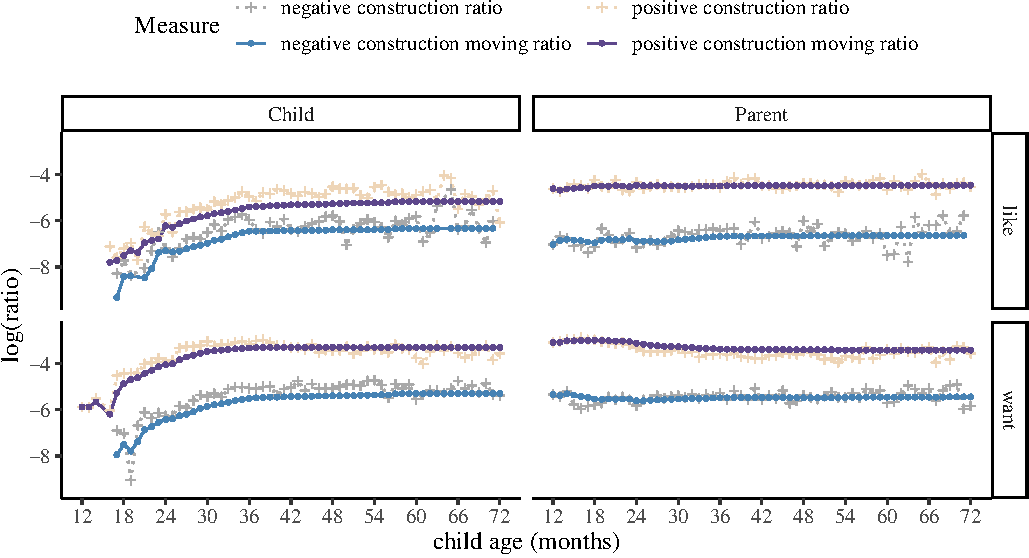
\includegraphics{neg_construction_article_files/figure-latex/emotion-1} 

}

\caption{Cumulative ratios for the production of rejection at the sentence level for children between 12 to 72 months of age, and their parents. The y-axes are scaled differently for the panels to accommodate differences in production ratios.}\label{fig:emotion}
\end{figure}

Starting with our analysis at the sentence level, Figure \ref{fig:emotion} shows the cumulative ratios of parents' and children's instances of rejections and their positive counterparts (y-axis) with age along the x-axis. Overall, we see a similar pattern of production for rejection whether the head verb is \emph{want} or \emph{like} in child speech. Comparing the cumulative ratios between parents and children, children's production of rejection gradually increases between the ages of 18 and 36 months. After about 36 months of age, children's production of these constructions starts to become relatively constant and close to parent levels. The main exception is positive instances with the head verb \emph{like}. Parents produced such constructions more frequently than children across at different ages. In all age bins, the production ratio for negative utterances was lower than that for their positive counterparts.

On the discourse level, we investigated discourse interactions (antecedent + utterance with negative discourse particle) in which the antecedent has one of the head verbs \emph{like} or \emph{want}, yet the head verb does not have to be modified by negative morphemes (Table \ref{tab:disreject}). We found a total of 11,021 such utterances (child: 7,903; parent: 3,118). As shown in Figure 2, children's production of \emph{no} to convey rejection increases regularly from the age of 18 - 36 months\footnote{For each communicative function, at the discourse level we also examined cases of different subtypes (e.g., different head verbs) separately; though due to data sparsity issues, we collapsed these instances for our final analyses.}. Overall, negation is produced at the discourse level more frequently in child speech compared to parent speech.

\begin{longtable}[]{@{}ll@{}}
\caption{\label{tab:disreject} Examples of discourse-level rejections in children's and parents' speech.}\tabularnewline
\toprule
Antecedent & Utterance \\
\midrule
\endfirsthead
\toprule
Antecedent & Utterance \\
\midrule
\endhead
Parent: \emph{I want you to try it} & Child: \emph{no no no} \\
Parent: \emph{would you like to go} & Child: \emph{no no} \\
Child: \emph{I don't like that} & Parent: \emph{no honey you have to try it} \\
Child: \emph{I want it} & Parent: \emph{no this is not for you} \\
\bottomrule
\end{longtable}

\begin{figure}[H]

{\centering 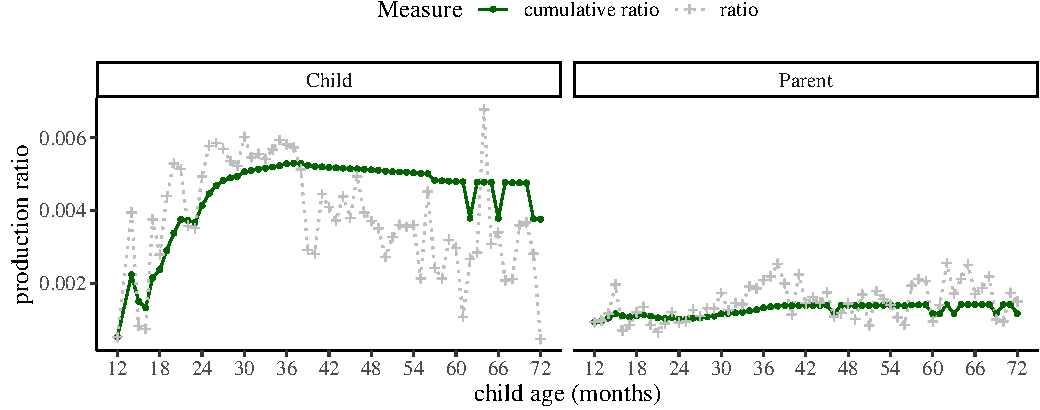
\includegraphics{neg_construction_article_files/figure-latex/emotiondiscourse-1} 

}

\caption{Cumulative ratios for the production of rejection at the discourse level for children between 12 to 72 months of age, and their parents.}\label{fig:emotiondiscourse}
\end{figure}

\hypertarget{non-existence}{%
\subsubsection{Non-existence}\label{non-existence}}

For the function of non-existence, we searched for the English expletive construction and extracted utterances that had \emph{there}-expletives, followed by a copula, and a noun phrase (phrases headed by either nouns or pronouns). We classified utterances where the predicate was modified by negation as negative, and the rest as positive. This led to a total of 1,983 negative utterances (child: 498; parent: 1,485), and 35,287 positive utterances (child: 8,385; parent: 26,902).

\begin{longtable}[]{@{}ll@{}}
\caption{\label{tab:nonexist} Examples of sentence-level non-existence and positive counterparts in children's speech.}\tabularnewline
\toprule
Non-existence (Negative) & Positive counterpart \\
\midrule
\endfirsthead
\toprule
Non-existence (Negative) & Positive counterpart \\
\midrule
\endhead
\emph{there's no (more) water} & \emph{there are books} \\
\emph{there isn't it} & \emph{there is it} \\
\emph{there's no more cheese} & \emph{there is the toy} \\
\emph{there is no food} & \emph{there is an apple} \\
\bottomrule
\end{longtable}

At the sentence level, children produced negative constructions to express non-existence less frequently than the positive counterparts. As Figure \ref{fig:existence} shows, the cumulative ratio for the production of non-existence increases mostly from 18 to 36 months. Then around and after 36 months of age, children's production gradually reaches a stable ratio but stays below parents' level. Notice that there appears to be slight fluctuations of cumulative ratios between the age of 19 and 25 months in child production. A closer inspection of the data reveals that within that age range, the frequency of negative utterances at most ages is either one or zero. Therefore as the number of total utterances increases along the developmental trajectory, the cumulative ratio for negative existential utterances actually decreases in this brief period.

\begin{figure}[H]

{\centering 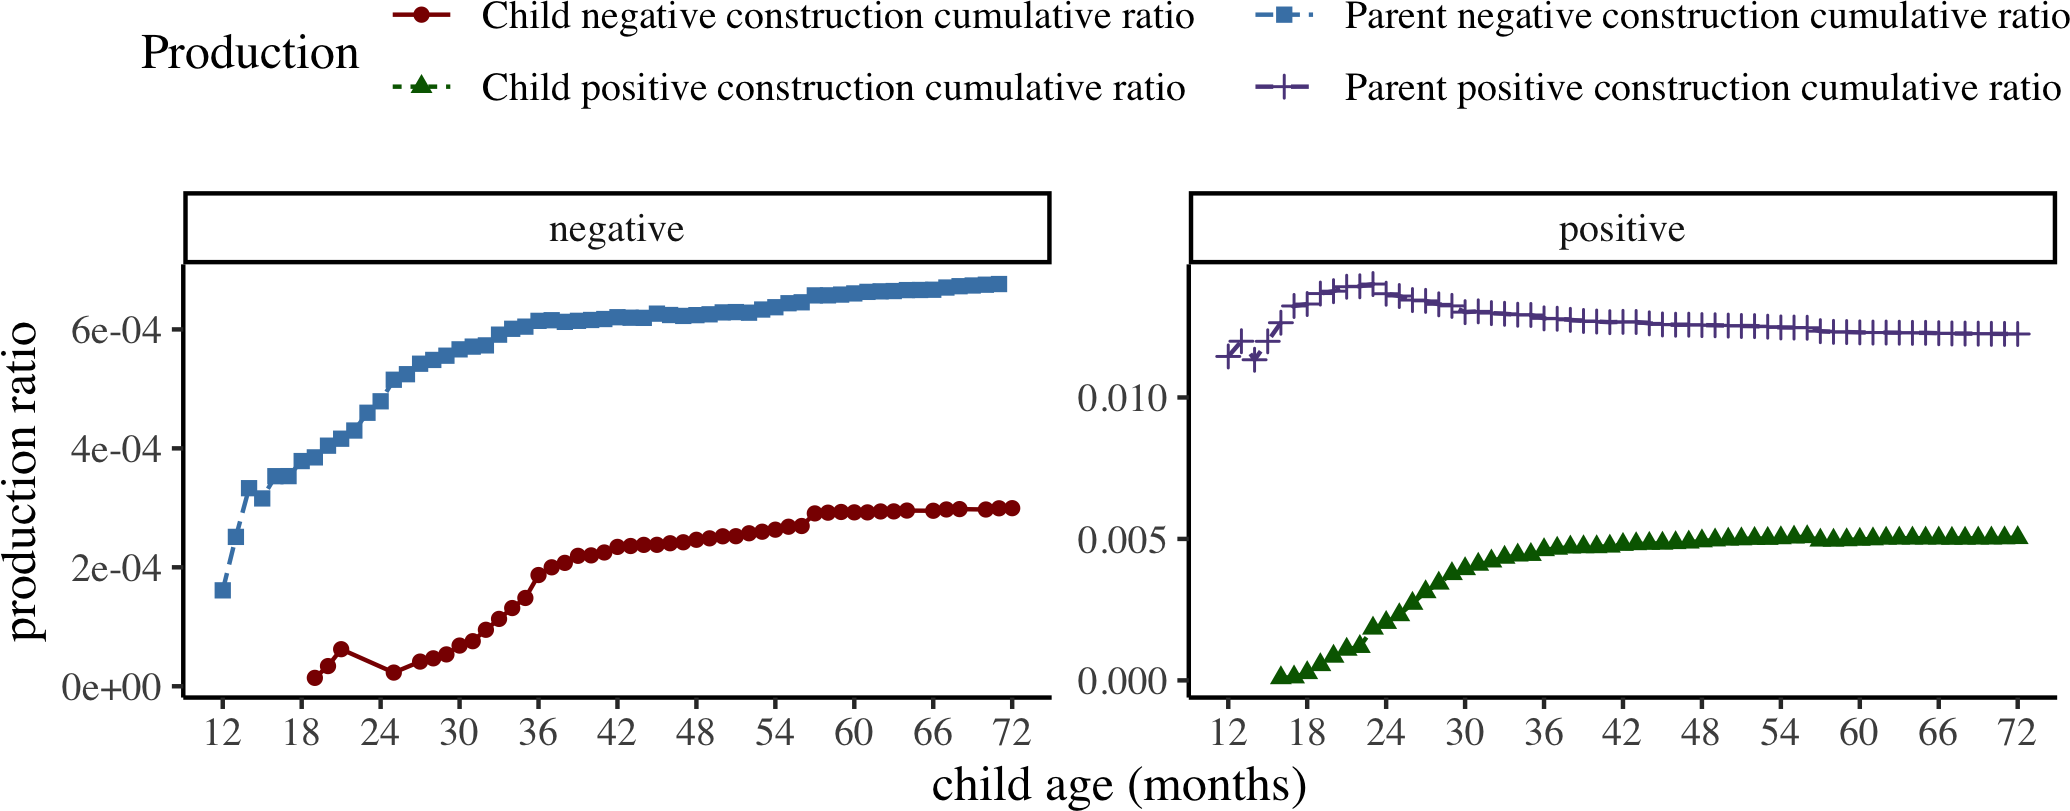
\includegraphics{neg_construction_article_files/figure-latex/existence-1} 

}

\caption{Cumulative ratios for the production of non-existence at the sentence level for children between 12 to 72 months of age, and their parents. The y-axes are scaled differently for the panels to accommodate differences in production ratios.}\label{fig:existence}
\end{figure}

For non-existence at the discourse level, we applied similar selection criteria and extracted utterances (negative and positive) with existential constructions in their antecedents (Table \ref{tab:disexist}). This led to a total of 1,202 utterances (child: 828; parent: 374). As Figure \ref{fig:existencediscourse} shows, there is an increase in children's responses with \emph{no} to parents' existential utterances between the ages of 18 and 36 months. After 36 months, despite the fact that ratios show fluctuations, the cumulative ratios of children's production seem stable and similar. Therefore with non-existence, both sentence level and discourse level analyses point to substantial development in the age rage of 18-36 months.

\begin{longtable}[]{@{}ll@{}}
\caption{\label{tab:disexist} Examples of discourse-level non-existence in children's and parents' speech.}\tabularnewline
\toprule
Antecedent & Utterance \\
\midrule
\endfirsthead
\toprule
Antecedent & Utterance \\
\midrule
\endhead
Parent: \emph{is there a bunny} & Child: \emph{no no bunny} \\
Parent: \emph{is there a table} & Child: \emph{no no} \\
Child: \emph{there is my ball} & Parent: \emph{no that's not yours} \\
Child: \emph{is there lunch bag} & Parent: \emph{no not yet sweety} \\
\bottomrule
\end{longtable}

\begin{figure}[H]

{\centering 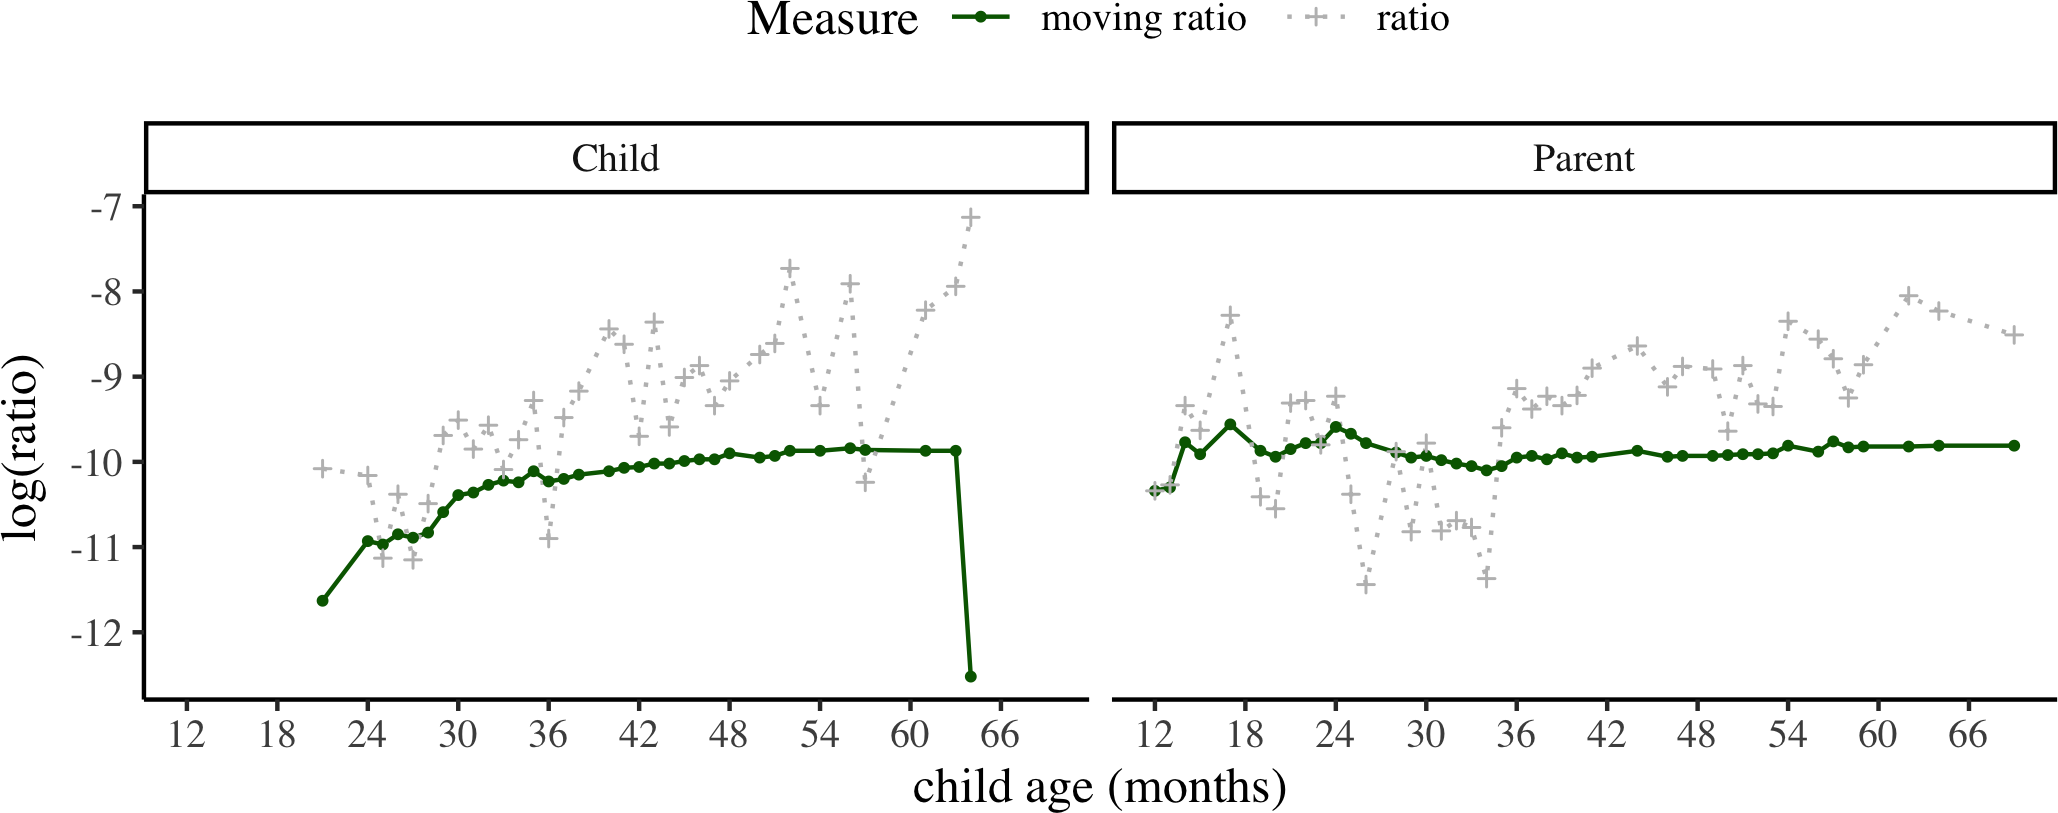
\includegraphics{neg_construction_article_files/figure-latex/existencediscourse-1} 

}

\caption{Cumulative ratios for the production of non-existence at the discourse level for children between 12 to 72 months of age, and their parents.}\label{fig:existencediscourse}
\end{figure}

\hypertarget{prohibition}{%
\subsubsection{Prohibition}\label{prohibition}}

For constructions that typically convey prohibition, we extracted utterances that were labeled as ``imperatives'' in the CHILDES database. In particular, we selected instances where the head verbs do not take any subjects. As before, cases without any negative morphemes are considered as positive. For negative constructions, we chose structures where the negative morphemes are combined with the auxiliary verb \emph{do} and they together modify the head verbs of the sentences. In order to not have overlap with rejection, non-existence, epistemic negation and possession (see Possession below), our search excluded utterances where the head verb had any of the following lemma forms: \emph{like}, \emph{want}, \emph{know}, \emph{think}, \emph{remember}, \emph{have}. This resulted in a total of 1,056 negative utterances (child: 303; parent: 753), and a total of 25,542 positive utterances (child: 8,659; parent: 16,883).

Figure \ref{fig:prohibition} shows the cumulative ratios of prohibitions and their positive counterparts in parents' and children's production at the sentence level. In both child and parent speech, negative constructions for prohibition are consistently produced less frequently than their positive counterparts. Children produce negative imperatives more and more often between 24 and 36 months. In comparison, the cumulative ratio in parent speech gradually decreases at the beginning when children are between 12 - 24 months. Yet overall, child production remains consistently lower than parent production of prohibition. This might be due to the social nature of parent-child interactions, in which it is more likely for parents to explicitly command and direct children's actions than the other way round.

\begin{longtable}[]{@{}ll@{}}
\caption{\label{tab:prohibit} Examples of sentence-level prohibition and positive counterparts in children's speech.}\tabularnewline
\toprule
Prohibition (Negative) & Positive counterpart \\
\midrule
\endfirsthead
\toprule
Prohibition (Negative) & Positive counterpart \\
\midrule
\endhead
\emph{don't blame Charlotte} & \emph{cook it} \\
\emph{don't do that} & \emph{try this} \\
\emph{do not touch that} & \emph{drink your water} \\
\emph{do not break it} & \emph{come here} \\
\bottomrule
\end{longtable}

\begin{figure}[H]

{\centering 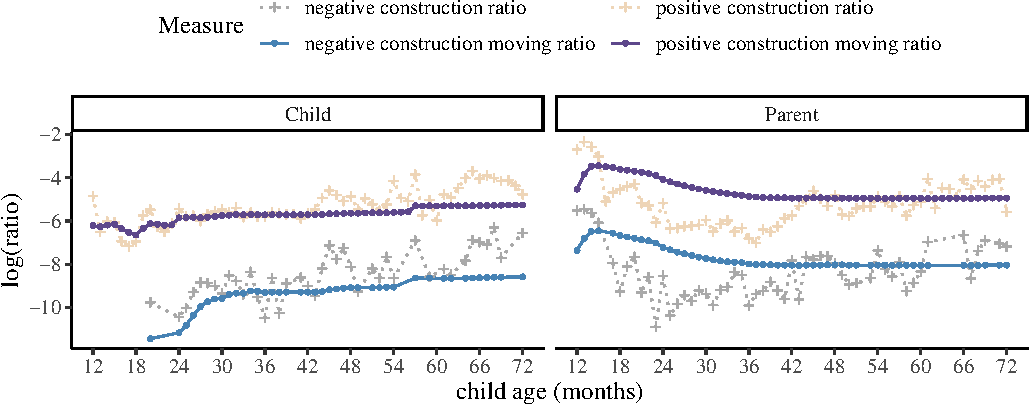
\includegraphics{neg_construction_article_files/figure-latex/prohibition-1} 

}

\caption{Cumulative ratios for the production of prohibition at the sentence level for children between 12 to 72 months of age, and their parents. The y-axes are scaled differently for the panels to accommodate differences in production ratios.}\label{fig:prohibition}
\end{figure}

At the discourse level, we selected utterances where \emph{no} serves as discourse response particle to antecedents that were subjectless imperatives headed by a verb. Again we excluded cases where the head verbs have any of the following lemmas: \emph{like}, \emph{want}, \emph{know}, \emph{think}, \emph{remember}, and \emph{have}. We would like to point out that in these instances, children's (and parents') production of \emph{no} is not necessarily negating the content of the antecedent prohibition. Instead we simply included these cases as lens to probing children's negative responses to imperatives, and also to be consistent with our analyses of the negative constructions of other communicative functions. Overall our search resulted in a total of 107 utterances (child: 65; parent: 42).
As shown in Figure \ref{fig:prohibitiondiscourse}, both children's and parents' usage of negation as a response particle to imperatives gradually decreases before 36 months, then stays relatively stable after. Nevertheless, given the extremely small sample size here, these observations are not conclusive.

\begin{longtable}[]{@{}ll@{}}
\caption{\label{tab:disprohib} Examples of discourse-level prohibition in children's and parents' speech.}\tabularnewline
\toprule
Antecedent & Utterance \\
\midrule
\endfirsthead
\toprule
Antecedent & Utterance \\
\midrule
\endhead
Parent: \emph{put away your toys} & Child: \emph{no mommy I like these} \\
Parent: \emph{don't put it there} & Child: \emph{no I really want to} \\
Child: \emph{give it to me} & Parent: \emph{no not right now} \\
Child: \emph{try it} & Parent: \emph{no no please} \\
\bottomrule
\end{longtable}

\begin{figure}[H]

{\centering 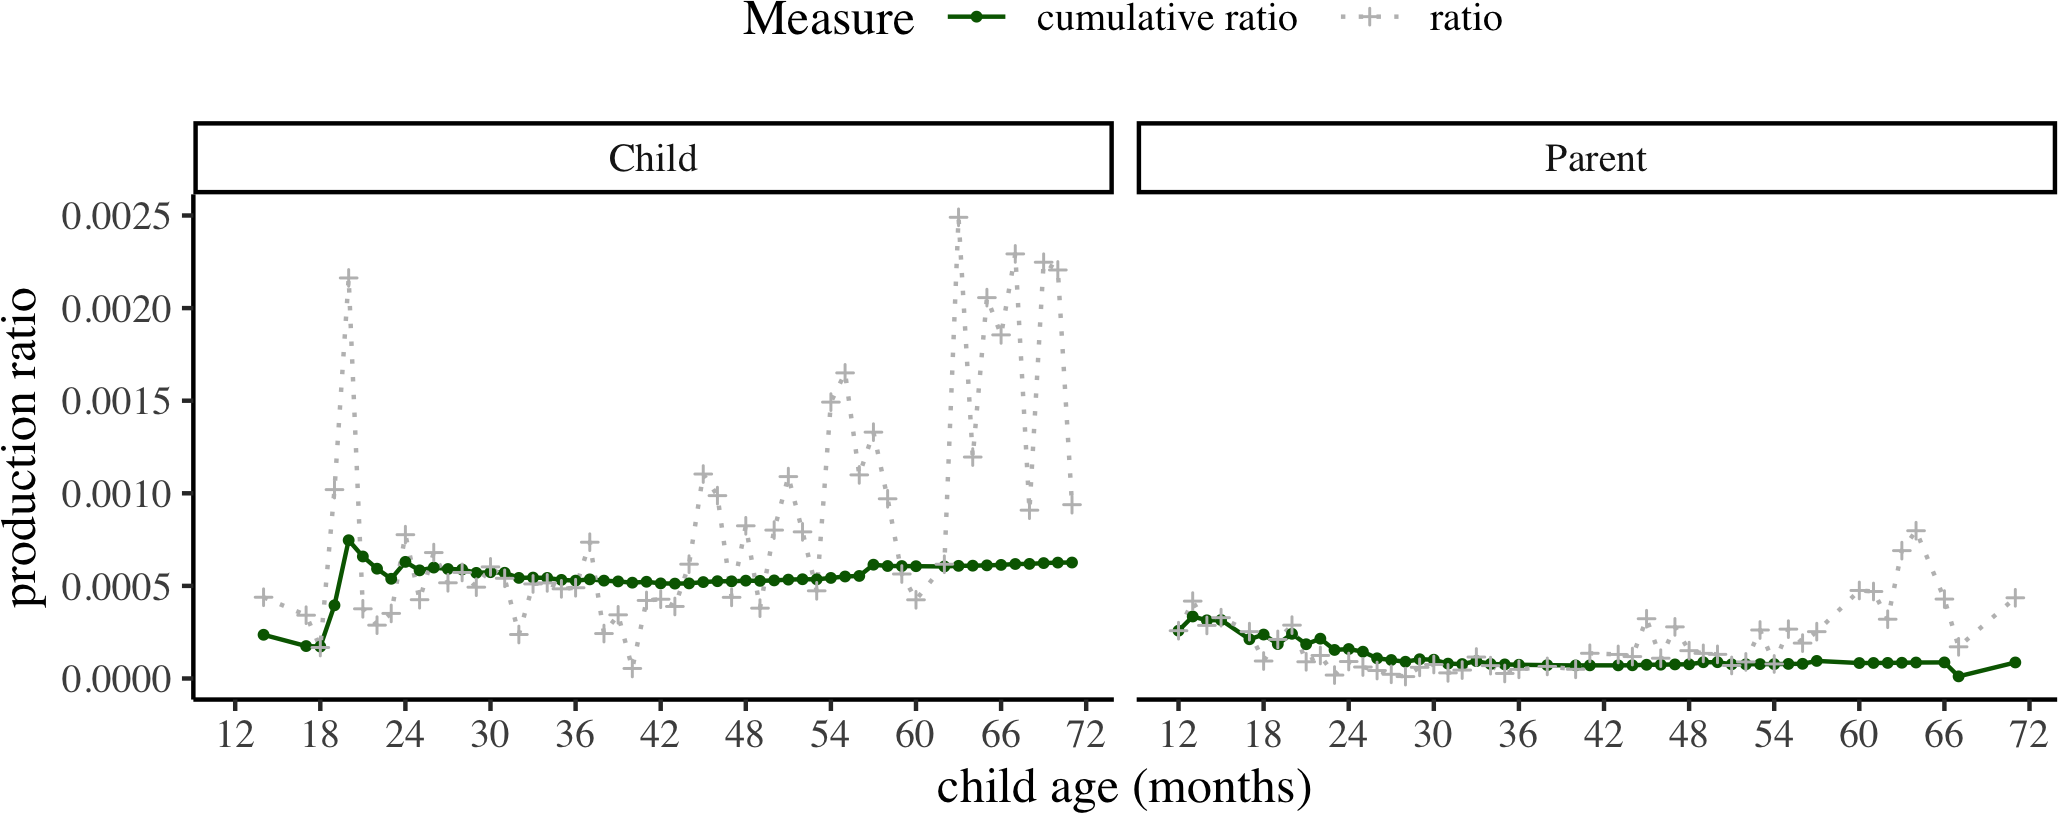
\includegraphics{neg_construction_article_files/figure-latex/prohibitiondiscourse-1} 

}

\caption{Cumulative ratios for the production of prohibition at the discourse level for children between 12 to 72 months of age, and their parents.}\label{fig:prohibitiondiscourse}
\end{figure}

\hypertarget{inability}{%
\subsubsection{Inability}\label{inability}}

For the function of inability, we analyzed instances with head verbs that are modified by the modal auxiliaries \emph{can} and \emph{could}. If the head verb was also modified by a negative morpheme, we classified it as negative. Otherwise, we considered it positive. Depending on the larger context, the interpretation of utterances such as ``can't go yet'' and ``this can't go in the box'' could be deontic (e.g., ``not allowed to go yet''). Given the automatic fashion of our approach, in order to limit the number of cases that potentially yield readings other than (in)ability, we excluded cases without a subject or with subjects that were not first person singular \emph{I}. This led to 7,115 negative utterances (child: 3,917; parent: 3,198), and 14,433 positive utterances (child: 7,589; parent: 6,844). Table \ref{tab:inab} shows a few example of the cases we considered.

\begin{longtable}[]{@{}ll@{}}
\caption{\label{tab:inab} Examples of sentence-level inability and positive counterparts in children's speech.}\tabularnewline
\toprule
Inability (Negative) & Positive counterpart \\
\midrule
\endfirsthead
\toprule
Inability (Negative) & Positive counterpart \\
\midrule
\endhead
\emph{I can't see} & \emph{I could do it} \\
\emph{I can't go} & \emph{I could help it} \\
\emph{I can not} & \emph{I can try} \\
\emph{I can not do it} & \emph{I can put it back} \\
\bottomrule
\end{longtable}

Figure \ref{fig:inability} shows cumulative ratios of parents and children's production of constructions that convey (in)ability. Similar to previous constructions, positive instances are generally more frequent than negative ones. Children produce inability more and more frequently between 18-36 months. After 36 months, their production is gradually becoming stable and higher than parents' production level.

\begin{figure}[H]

{\centering 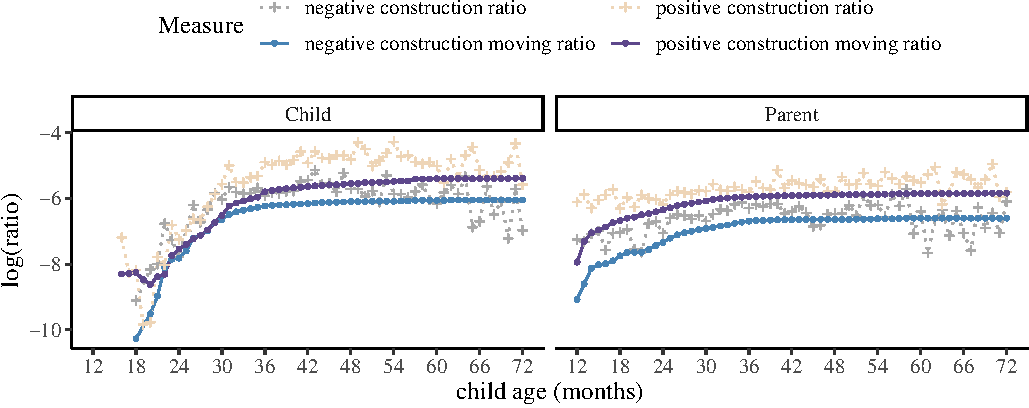
\includegraphics{neg_construction_article_files/figure-latex/inability-1} 

}

\caption{Cumulative ratios for the production of inability at the sentence level for children between 12 to 72 months of age, and their parents. The y-axes are scaled differently for the panels to accommodate differences in production ratios.}\label{fig:inability}
\end{figure}

\begin{longtable}[]{@{}ll@{}}
\caption{\label{tab:disinability} Examples of discourse-level inability in children's and parents' speech.}\tabularnewline
\toprule
Antecedent & Utterance \\
\midrule
\endfirsthead
\toprule
Antecedent & Utterance \\
\midrule
\endhead
Parent: \emph{I can do it for you} & Child: \emph{no no} \\
Parent: \emph{I can't see} & Child: \emph{no try again} \\
Child: \emph{I can pour this} & Parent: \emph{no no please} \\
Child: \emph{I can't finish} & Parent: \emph{no you have to} \\
\bottomrule
\end{longtable}

At the discourse level, we chose utterances with the negative particle \emph{no} in response to antecedents that had a similar structure to the inability construction defined at the sentence level. In these interatctions, \emph{no} is not exactly negating the content of the antecedents neither; however, similarly to our motivation for analyzing prohibition at the discourse level, we included these instances to investigate children's (and parents') negative response to (in)ability more broadly. This yielded a total of 1,275 negative utterances (child: 621; parent: 654). Figure \ref{fig:inabilitydiscourse} shows the ratios and the cumulative ratios for parents' and children's production of discourse level inability construction. Considering cumulative ratios, children's production gradually increases from 24 to 36 months and stabalizes after 36 months at a similar rate to that of parent's.

\begin{figure}[H]

{\centering 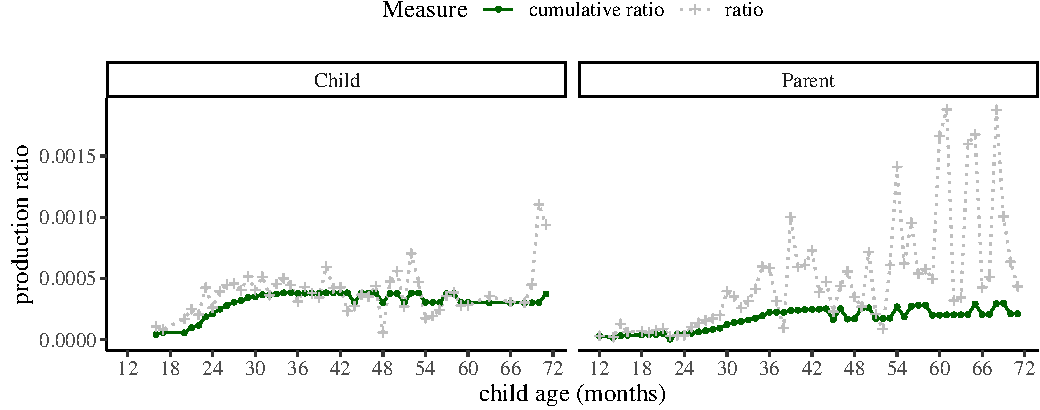
\includegraphics{neg_construction_article_files/figure-latex/inabilitydiscourse-1} 

}

\caption{Cumulative ratios for the production of inability at the discourse level for children between 12 to 72 months of age, and their parents.}\label{fig:inabilitydiscourse}
\end{figure}

\hypertarget{labeling}{%
\subsubsection{Labeling}\label{labeling}}

To capture the function of labeling at the sentence level, we concentrated on copula structures in which the predicate is a nominal or an adjectival phrase. Specifically, the nominal predicates exclude possessive pronouns (e.g., ``mine'') as well as nominals with a possessive dependent (e.g., ``my book'') in order to not overlap with the communicative function of possession (see Possession below). We considered instances where the predicate is modified by negative morphemes as negative, and others as positive. To also avoid overlap with cases of non-existence, none of the utterances contained expletives (e.g., ``there is no book''). This resulted in a total of 36,410 negative utterances (Child: 6,193; Parent: 30,217), and 484,679 positive utterances (Child: 121,107; Parent: 363,572).

\begin{longtable}[]{@{}ll@{}}
\caption{\label{tab:label} Examples of sentence-level labeling (negative) and positive counterparts in children's speech.}\tabularnewline
\toprule
Labeling (Negative) & Positive counterpart \\
\midrule
\endfirsthead
\toprule
Labeling (Negative) & Positive counterpart \\
\midrule
\endhead
\emph{that's not a farmer} & \emph{this is a book} \\
\emph{this is not the book} & \emph{this is nice} \\
\emph{I'm not a heavy baby Mum} & \emph{it's a nice bowl} \\
\emph{It's no good} & \emph{she's pretty} \\
\bottomrule
\end{longtable}

Figure \ref{fig:learning} shows cumulative ratios for parent's and children's production of the labeling construction at the sentence level. In both parent and children speech, the frequency of positive counterparts is consistently higher than that of negative labeling instances. Children's production of negative labeling increases between 18-36 months, and remains stable after then; though the production ratios remained lower than those of parents' production.

\begin{figure}[H]

{\centering 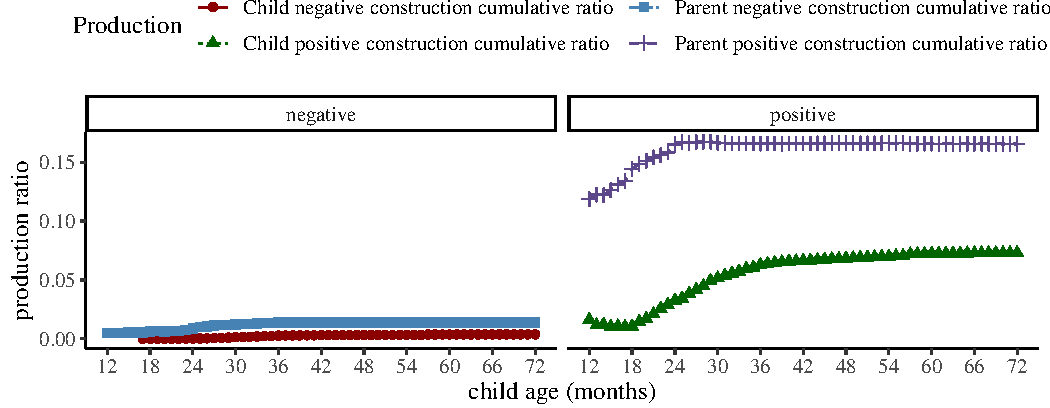
\includegraphics{neg_construction_article_files/figure-latex/learning-1} 

}

\caption{Cumulative ratios for the production of (negative) labeling at the sentence level for children between 12 to 72 months of age, and their parents. The y-axes are scaled differently for the panels to accommodate differences in production ratios.}\label{fig:learning}
\end{figure}

At the discourse level, we selected antecedent utterances with copula structures that combined with a nominal or an adjectival predicate (\ref{tab:dislabel}). In total we found 18,037 utterances (Child: 12,501; Parent: 5,536). Figure \ref{fig:learningdiscourse} shows the cumulative ratios for labeling instances at the discourse level. There is an increase in children use of \emph{no} to negate labeling between 18 to 36 months. After 36 months, however, the production stays at a stable rate above parents level.

\begin{longtable}[]{@{}ll@{}}
\caption{\label{tab:dislabel} Examples of discourse-level labeling (negative) in children's and parents' speech.}\tabularnewline
\toprule
Antecedent & Utterance \\
\midrule
\endfirsthead
\toprule
Antecedent & Utterance \\
\midrule
\endhead
Parent: \emph{is this one good} & Child: \emph{no it's not} \\
Parent: \emph{are you a captain} & Child: \emph{no I'm not} \\
Child: \emph{that's the one} & Parent: \emph{no it's the green one} \\
Child: \emph{this is the key} & Parent: \emph{no no} \\
\bottomrule
\end{longtable}

\begin{figure}[H]

{\centering 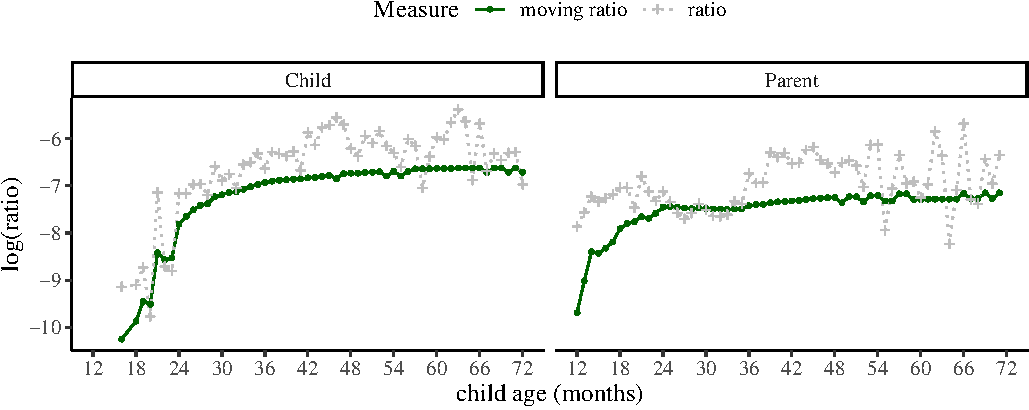
\includegraphics{neg_construction_article_files/figure-latex/learningdiscourse-1} 

}

\caption{Cumulative ratios for the production of (negative) labeling at the discourse level for children between 12 to 72 months of age, and their parents.}\label{fig:learningdiscourse}
\end{figure}

\hypertarget{epistemic-negation}{%
\subsubsection{Epistemic Negation}\label{epistemic-negation}}

Previous studies have reported instances in which children combined negative morphemes with mental state verbs such as \emph{know}, \emph{think}, and \emph{remember} to express ``epistemic negation'' (Choi, 1988). To define epistemic constructions, we also focused on these three verbs. For sentence level epistemic negation, we analyzed negative utterances where these verbs were modified by negative morphemes, possibly after combining with an auxiliary verb like \emph{do}. Table \ref{tab:epistem} shows a few examples. Instances where the speaker asked about or described the negative epistemic state of another speaker were also included, leading to 31,696 negative utterances in total (child: 9,852; parent: 21,844). For the positive counterparts, we selected instances with the same head verbs except that these verbs were not modified by negation. This resulted in a total of 95,679 positive utterances (child: 16,322; parent: 79,357).

\begin{longtable}[]{@{}ll@{}}
\caption{\label{tab:epistem} Examples of sentence-level epistemic negation and positive counterparts in children's speech.}\tabularnewline
\toprule
Epistemic (Negative) & Positive counterpart \\
\midrule
\endfirsthead
\toprule
Epistemic (Negative) & Positive counterpart \\
\midrule
\endhead
\emph{I not know} & \emph{I know} \\
\emph{I didn't remember} & \emph{she remembers} \\
\emph{I don't think so} & \emph{he thinks this one is good} \\
\emph{She doesn't know this} & \emph{She knows about this} \\
\bottomrule
\end{longtable}

Figure \ref{fig:epistemic} shows the cumulative ratios of the epistemic construction as defined above in parents' and children's speech at the sentence level. Across the three head verbs, children's production increases substantially from 18 to 36 months then gradually becomes stable yet still lower than parents' production level afterwards. The number of epistemic instances headed by \emph{know} is overall higher than the number of cases headed by either \emph{remember} or \emph{think}, an observation that is consistent in both negative constructions and positive counterparts. With that being said, the majority of negative constructions headed by \emph{know} are idiomatic expressions such as ``I don't know'' (51.66\%) or ``don't know'' (13.73\%). Positive epistemic utterances are in general more frequent than negative ones, with the exception of with the exception of \emph{know} in child speech. Across the three head verbs, children's production with \emph{know} gradually approaches that of parents' around 30 - 36 months, whereas cases with the head verb \emph{remember} and \emph{think} are produced less frequently by children.

\begin{figure}[H]

{\centering 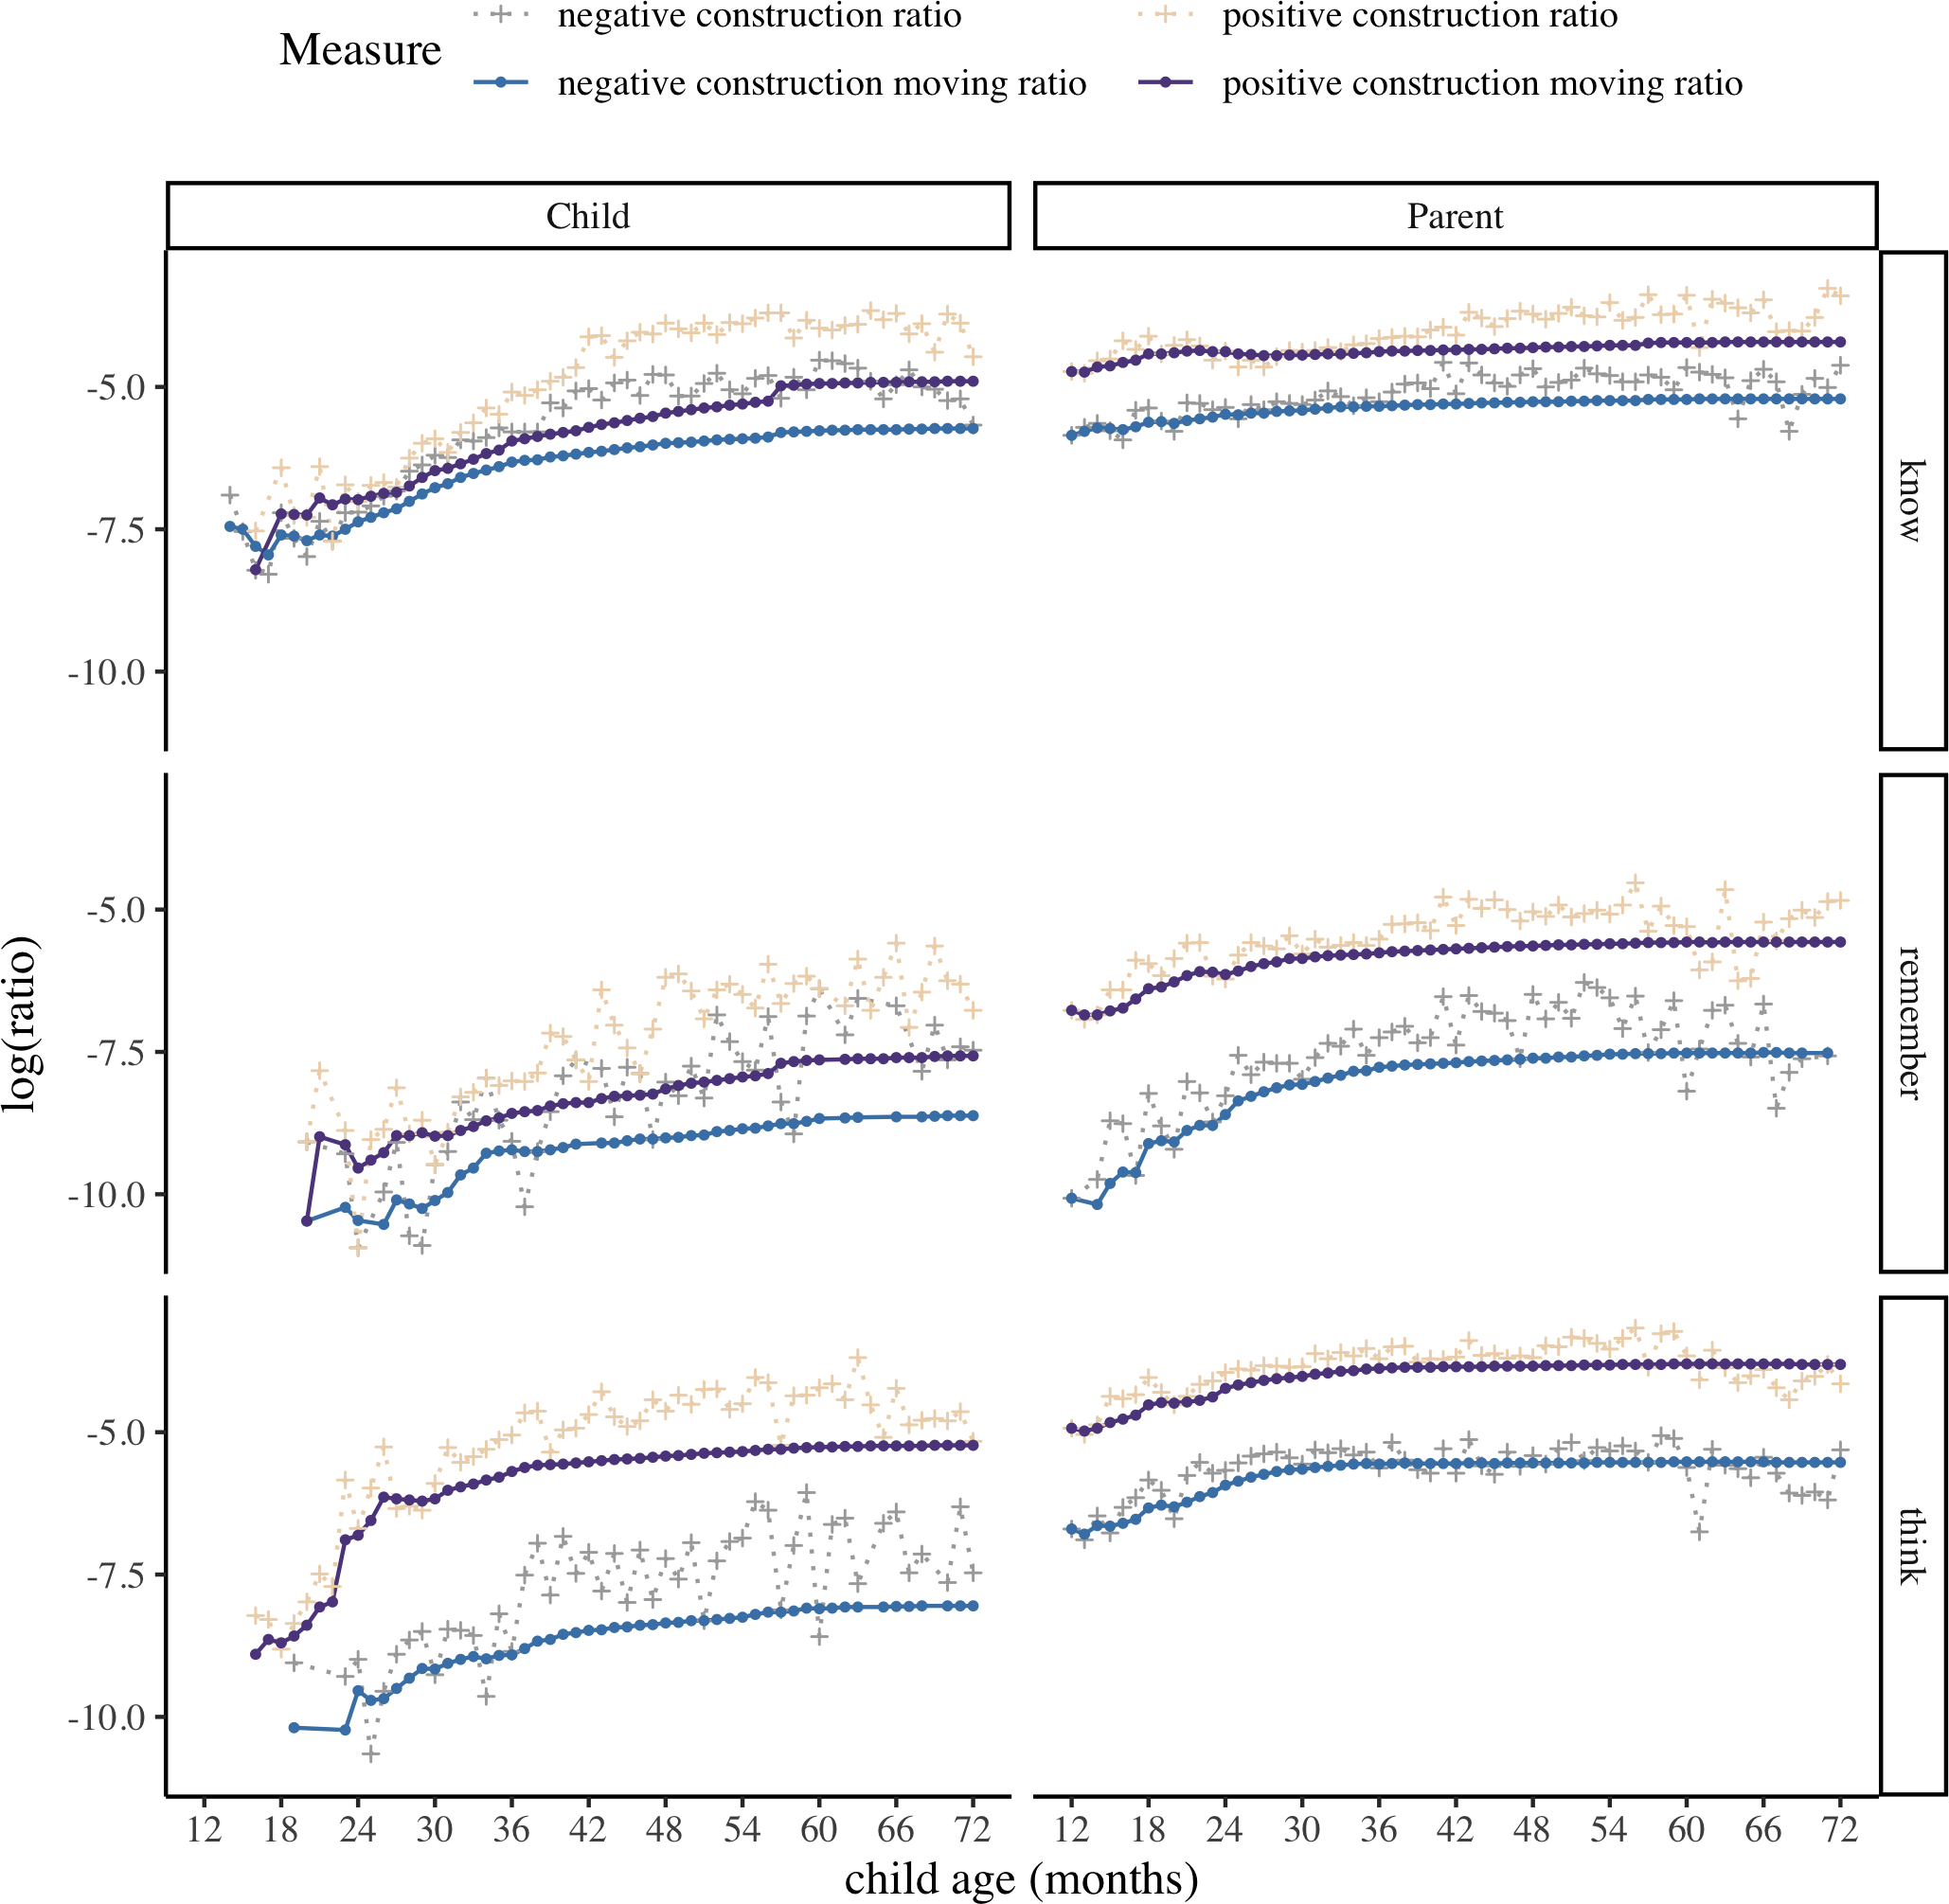
\includegraphics{neg_construction_article_files/figure-latex/epistemic-1} 

}

\caption{Cumulative ratios for the production of epistemic negation at the sentence level for children between 12 to 72 months of age, and their parents. The y-axes are scaled differently for the panels to accommodate differences in production ratios.}\label{fig:epistemic}
\end{figure}

For epistemic negation at the discourse level, we examined interactions in which the antecedent utterances took any of the three head verbs: \emph{know}, \emph{remember} and \emph{think}, leading to a total of 5,695 utterances (child: 4,303; parent: 1,392). As shown in Figure \ref{fig:epistemicdiscourse}, children's production of \emph{no} to negate antecedent epistemic utterances increases rapidly between 18-36 months and is in general higher than the production ratio of parents'.

\begin{longtable}[]{@{}ll@{}}
\caption{\label{tab:epistem} Examples of discourse-level epistemic negation in children's and parents' speech.}\tabularnewline
\toprule
Epistemic (Negative) & Positive counterpart \\
\midrule
\endfirsthead
\toprule
Epistemic (Negative) & Positive counterpart \\
\midrule
\endhead
Parent: \emph{do you know} & Child: \emph{no} \\
Parent: \emph{do you remember} & \emph{no I don't remember it} \\
Child: \emph{does she think so} & Parent: \emph{no not really} \\
Child: \emph{do they know it's today} & \emph{no I don't think so honey} \\
\bottomrule
\end{longtable}

\begin{figure}[H]

{\centering 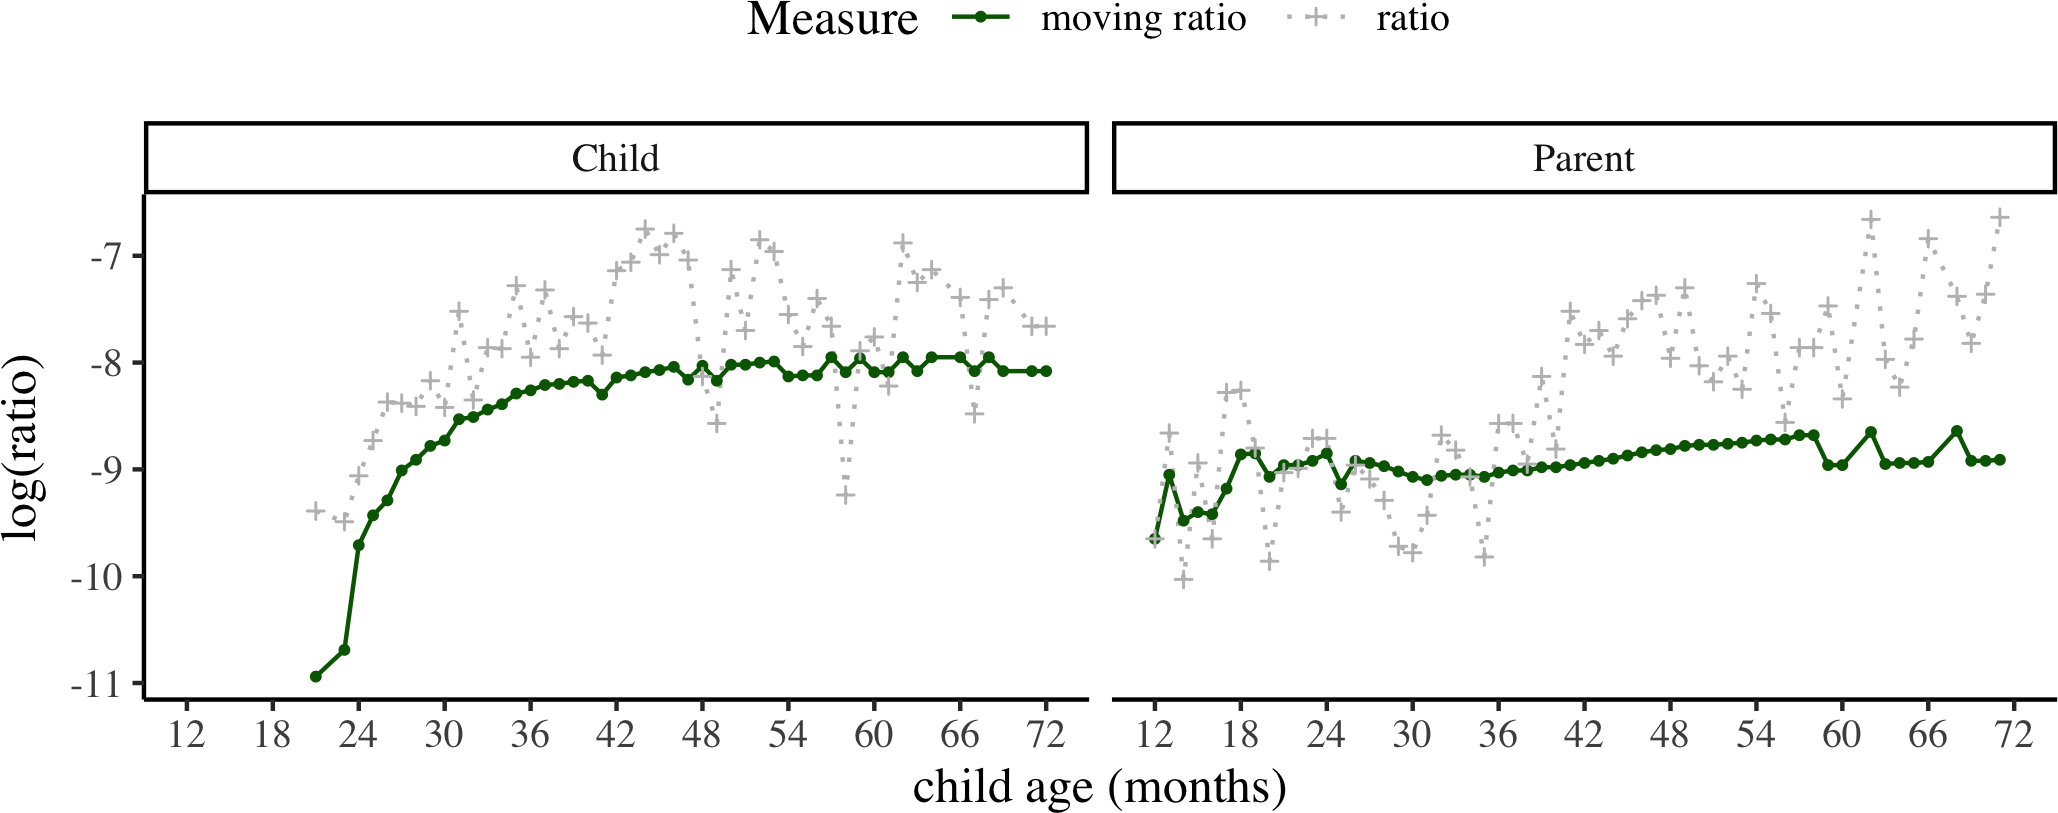
\includegraphics{neg_construction_article_files/figure-latex/epistemicdiscourse-1} 

}

\caption{Cumulative ratios for the production of epistemic negation at the discourse level for children between 12 to 72 months of age, and their parents.}\label{fig:epistemicdiscourse}
\end{figure}

\hypertarget{possession}{%
\subsubsection{Possession}\label{possession}}

The last function we explored was possession. At the sentence level, for negative structures we selected cases where negative morphemes were combined with auxiliary verbs to modify head verbs with the lemma form \emph{have}, and the POS tag of these head verbs is all VERB. We also included cases of which the syntactic head is a nominal predicate; the nominal predicate can either be a possessive pronoun (e.g., ``yours'') or a noun phrase with a possessive modifier (e.g., ``her book''). Table \ref{tab:possess} presents a few examples. The number of negative utterances subjected to analysis for this function is 8,892 (child: 2,830; parent: 6,062). Again the positive counterparts share similar structures except with no negation, leading to a total of 86,665 utterances (child: 27,730; parent: 58,935). One thing to note here is that for the positive structures with the head verb \emph{have}, we restricted our search to instances where the head verb takes a direct object (with the dependency relation \emph{obj}). This is to avoid potential parsing errors of utterances such as \emph{I have}, where the verb could ambiguously be an auxiliary.

\begin{longtable}[]{@{}ll@{}}
\caption{\label{tab:possess} Examples of sentence-level possession (negative) and positive counterparts in children's speech.}\tabularnewline
\toprule
Posession (Negative) & Positive counterpart \\
\midrule
\endfirsthead
\toprule
Posession (Negative) & Positive counterpart \\
\midrule
\endhead
\emph{I don't have it} & \emph{you have that} \\
\emph{you don't have my toy car} & \emph{she has it} \\
\emph{not mine} & \emph{this is hers} \\
\emph{not yours either} & \emph{mine mine mine} \\
\bottomrule
\end{longtable}

Figure \ref{fig:possession} presents cumulative ratios of possession construction at the sentence level. Regardless of whether the utterances are negative or positive, the production trajectory in child speech appears to have notable differences depending on what the syntactic head. When the instances are headed by \emph{have}, children increase their production between 18-36 months, a pattern that is present in both negative and positive constructions; yet children's production ratio consistently stays below parents' level across the developmental path. For utterances headed by possessive pronouns, on the other hand, children's production increases rapidly between 18-24 months and stays above parents' production level as early as 24 months of age.

\begin{figure}[H]

{\centering 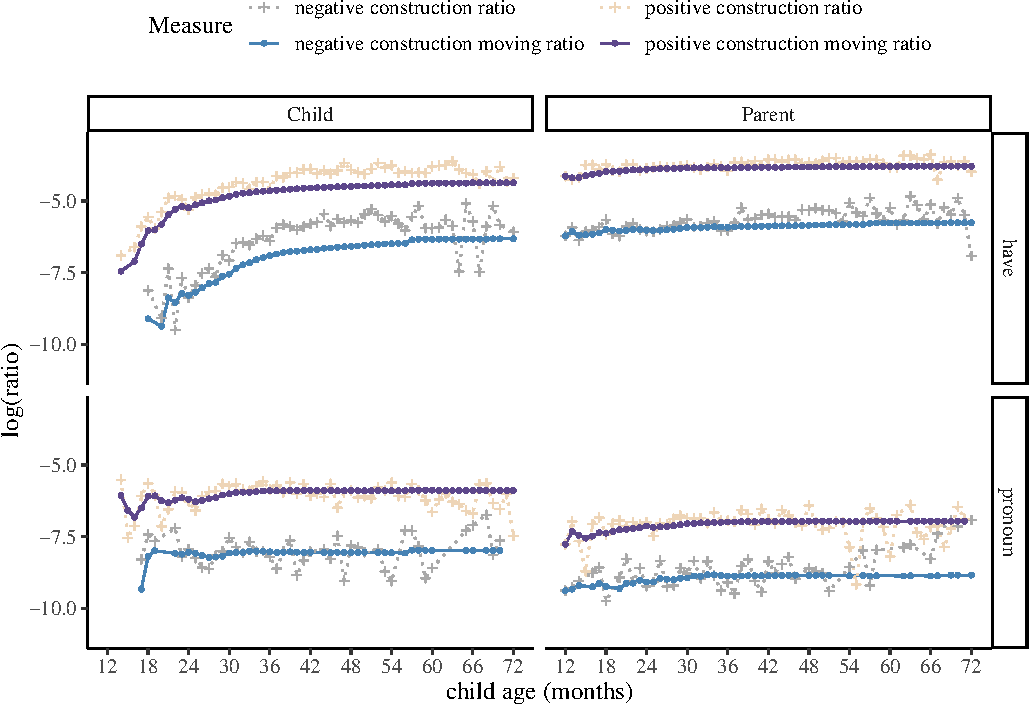
\includegraphics{neg_construction_article_files/figure-latex/possession-1} 

}

\caption{Cumulative ratios for the production of possession at the sentence level for children between 12 to 72 months of age, and their parents. The y-axes are scaled differently for the panels to accommodate differences in production ratios.}\label{fig:possession}
\end{figure}

For discourse level possessives, we selected antecedents of the negative response particle \emph{no} which themselves had structures similar to the negative and positive constructions of possession at the sentence level (Table \ref{tab:dispossess}). Based on Figure \ref{fig:possessiondiscourse}, the overall patterns indicate that children's production of discourse level possession increases gradually within the age range of 18 to 36 months; and their production ratio is mostly higher than that of parents.

\begin{longtable}[]{@{}ll@{}}
\caption{\label{tab:dispossess} Examples of discourse-level possession (negative) in children's and parents' speech.}\tabularnewline
\toprule
Antecedent & Utterance \\
\midrule
\endfirsthead
\toprule
Antecedent & Utterance \\
\midrule
\endhead
Parent: \emph{not yours} & Child: \emph{no it's mine mine} \\
Parent: \emph{do you still have that picture} & Child: \emph{no} \\
Child: \emph{I don't have the book} & Parent: \emph{no no mommy please read it to me} \\
Child: \emph{mommy has it} & Parent: \emph{no mommy gave it back to your auntie} \\
\bottomrule
\end{longtable}

\begin{figure}[H]

{\centering 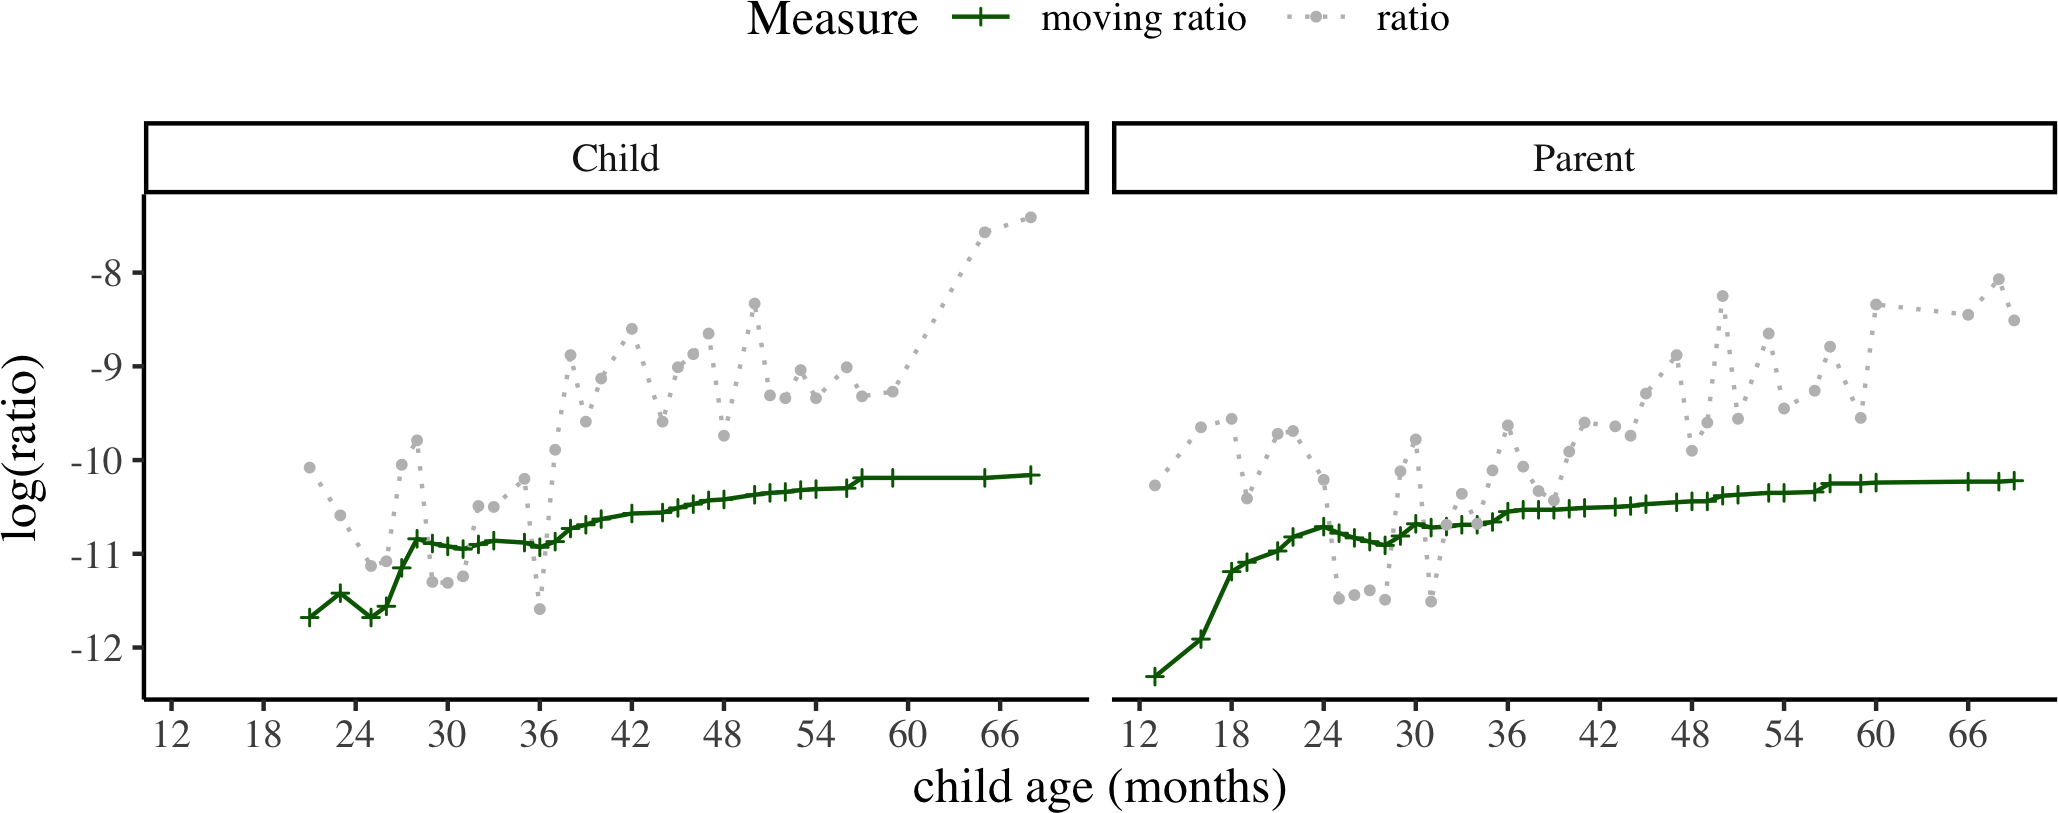
\includegraphics{neg_construction_article_files/figure-latex/possessiondiscourse-1} 

}

\caption{Cumulative ratios for the production of possession at the discourse level for children between 12 to 72 months of age, and their parents.}\label{fig:possessiondiscourse}
\end{figure}

\hypertarget{analysis-and-discussion}{%
\subsubsection{Analysis and Discussion}\label{analysis-and-discussion}}

Figure \ref{fig:allneg} shows the cumulative ratios of all our negative constructions at the sentence level for children (left panel) and parents (right panel).
It seems that parents produce most negative constructions at relatively constant rates across most of the age bins. Notable exceptions are labeling, epistemic, and prohibitions between 12-36 months. Parents seem to increase their production of labeling and epistemic constructions in this period and their production becomes more stable after 36 months. This obervation aligns with labeling and epistemic negation in child speech, which suggests that the production patterns in child speech for these two functions may be more influenced by interactions with parents, and vice versa as children grow to be more conversant and interactive. On the other hand, prohibition starts as one of the most frequent constructions at 12-18 months of age and ends up as the least frequently used construction after around 30 months. One obvious reason for this trend may be that when children are younger, parents guide their actions through imperatives and commands much more frequently than later in the child's life.

By comparison, children start producing most constructions in the 12-18 age range. Two constructions, non-existence and prohibition, seem to show some delay. With non-existence, even though there are examples between 18-24 months, the cumulative production ratios are fluctuating and discontinuous, instead of demonstrating a slow and steady increase as seen in most of the other functions. As described in previous sections, the data for non-existence before 25 months based on our corpus search is relatively sparse; it is possible that with more examples a clearer pattern may emerge. With prohibition, we see a relatively smooth pattern. Children begin to produce them later than other functions (more regularly between 24-30 months) and its rate of production stays below parents' levels. It is possible that parent-child interactions do not provide many contexts for children to prohibit parents. Overall by 36 months of age, children's production of most constructions starts to become stable.

\begin{figure}[H]

{\centering 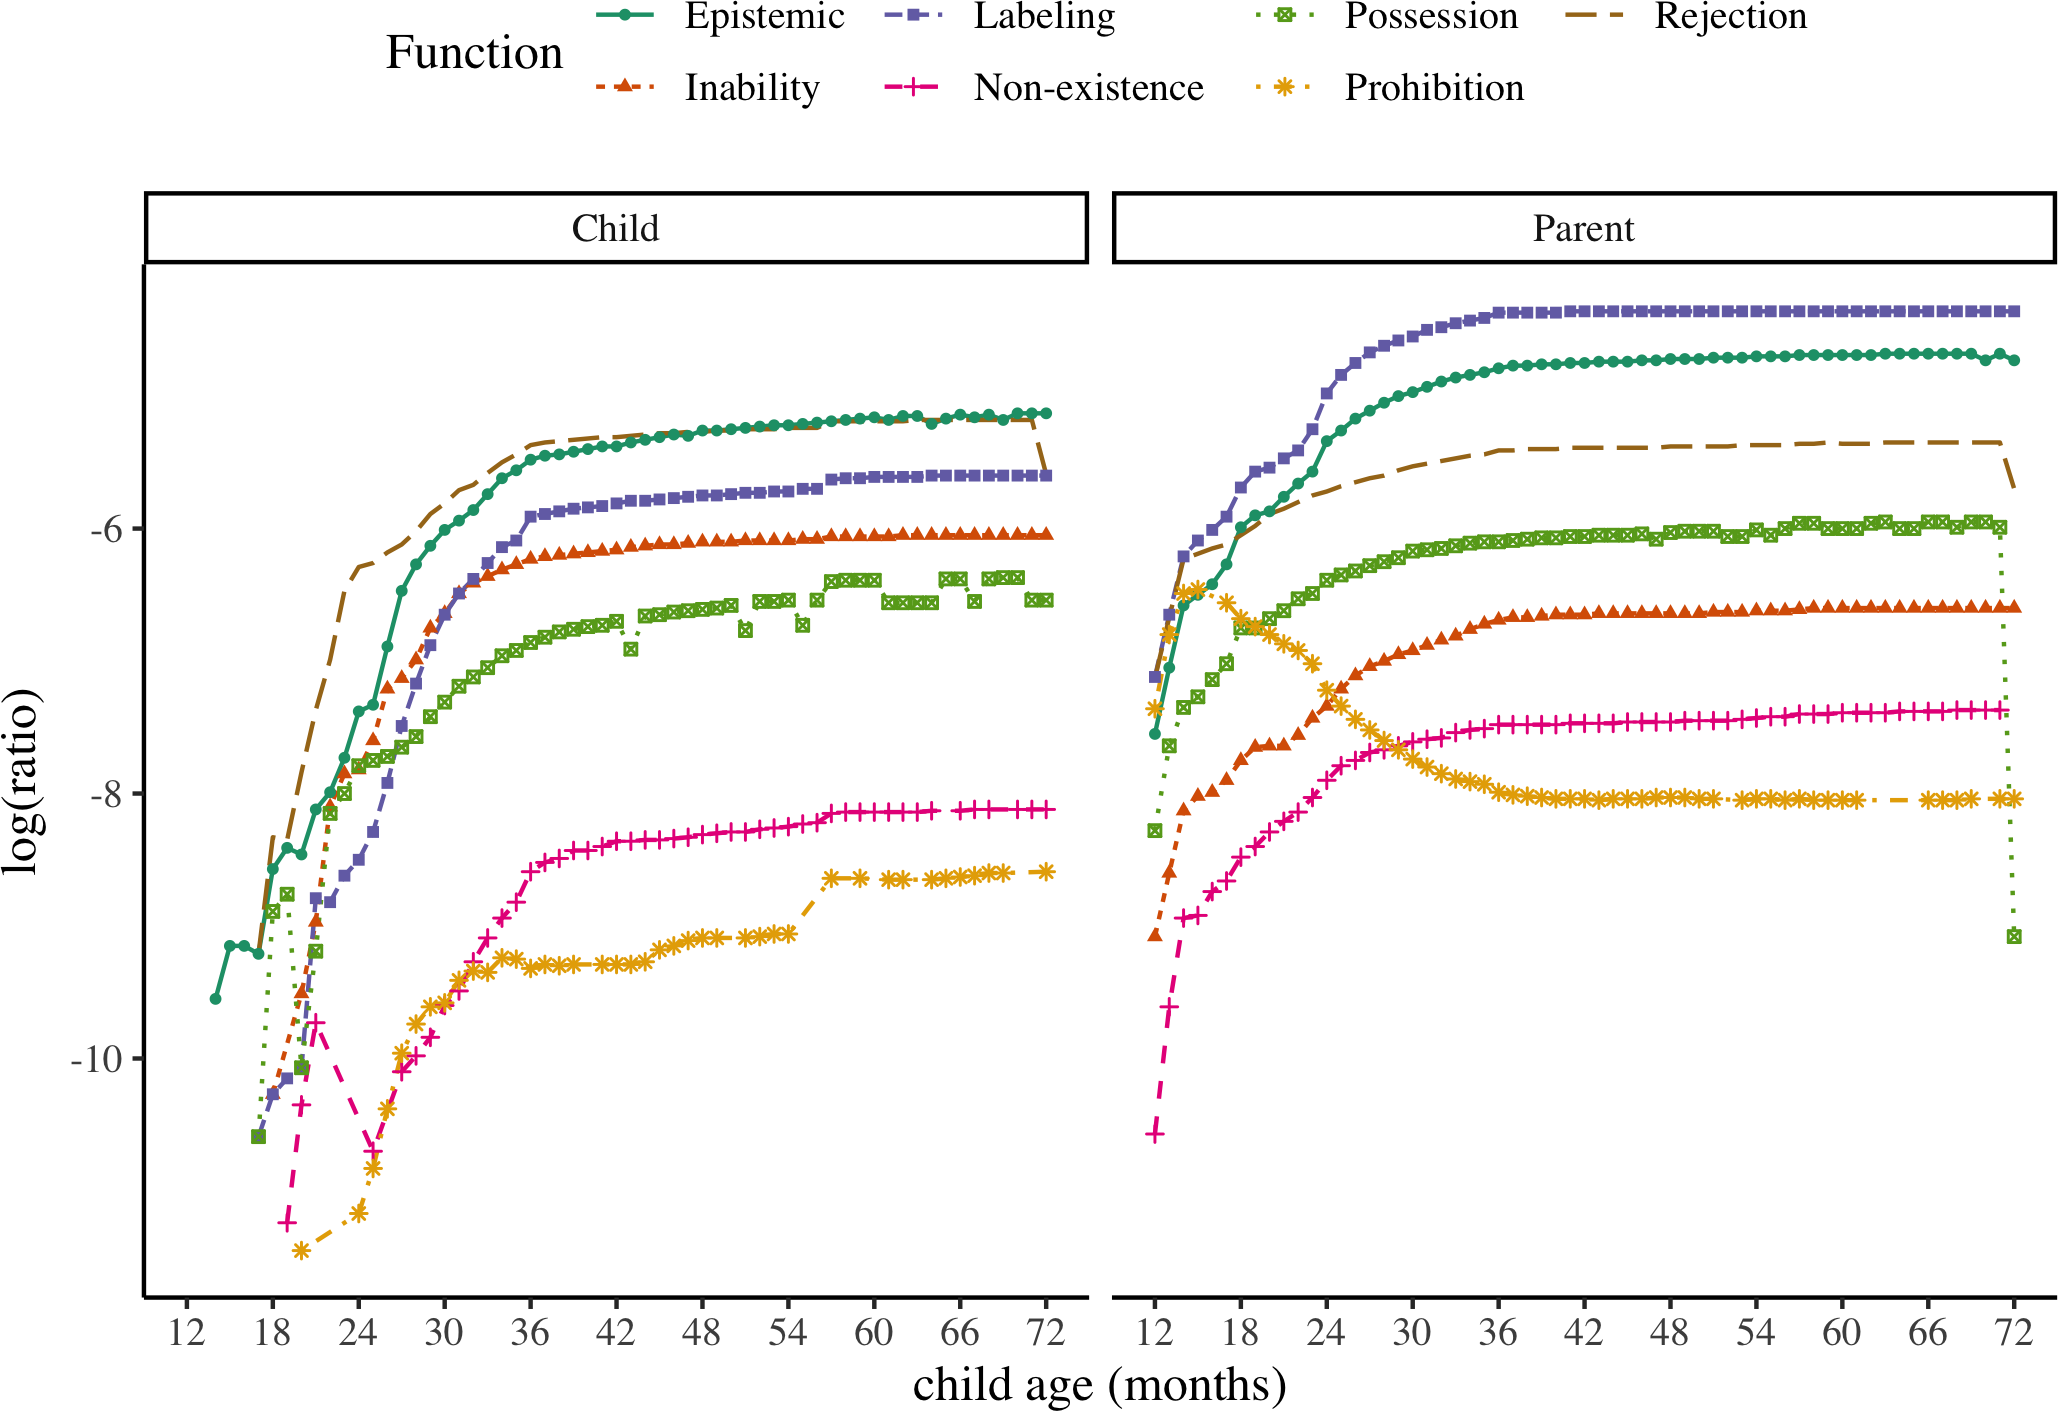
\includegraphics{neg_construction_article_files/figure-latex/allneg-1} 

}

\caption{Cumulative ratios for all negative constructions at the sentence level.}\label{fig:allneg}
\end{figure}

Figure \ref{fig:allpos} shows the cumulative ratios of all positive counterparts to our negative constructions at the sentence level for children (left panel) and parents (right panel). The production of the positive instances in parent speech for almost all constructions is stable and constant. Notable exceptions are labeling and positive counterparts to prohibitions (positive imperatives) between 12-30 months. Similar to negative instances of labeling, positive instances increase in frequency between 12-30 months but stay stable and constant after. Positive prohibitions are produced much more frequently at the beginning and between 12-36 months, but their production decreases later. This pattern mirrors what we see in Figure \ref{fig:allneg} with (negative) prohibitions, that the usage of imperatives in interactions potentially becomes less necessary as children grow older.

Compared to parent speech, children start producing all positive counterparts to our negative constructions between the age range of 12-18 months. By 36 months, almost all positive constructions are being produced at a relatively constant rate close to parents' levels. Another noteworthy pattern is the relative high frequency of positive counterparts to prohibitions in the 12-24 months age period. Unlike (negative) prohibitions that were produced with some delay (compared to other constructions) around 24-30 months, positive imperatives are produced with high frequency even before 24 months of age. In other words, even though children do not frequently prohibit parents, they seem to be frequently ordering or commanding parents to do things for them; a conclusion that may not surprise many parents or caregivers.

Summarzing children's production patterns at the sentence level, it appears that regardless of whether the utterance is negative or positive, there is considerable similarity in terms of the developmental trajectories across the different communicative functions. Though there are discrepancies for cases of prohibition, overall the development of most negative constructions and their positive counterparts emerges between 12-18 months; their production increases substantially from 18 to 36 months, then starts to become stable (increase very slowly) after 36 months of age. That the developmental path for each function is comparable is additionally evident from results of the Bayesian logistic growth curve modeling, shown in Table \ref{tab:growthsyntax}. Minus the precise numerical values, the production of the negative utterances for all communicative function is estimated to reach a similar asymtotic level, without statistically significant differences between each other. The maximum growth rate as well as the age at which one-half of production is achieved are also comparable across functions, despite of whether the construciton is negative.

\begin{longtable}[]{@{}
  >{\raggedright\arraybackslash}p{(\columnwidth - 10\tabcolsep) * \real{0.16}}
  >{\raggedright\arraybackslash}p{(\columnwidth - 10\tabcolsep) * \real{0.11}}
  >{\raggedright\arraybackslash}p{(\columnwidth - 10\tabcolsep) * \real{0.24}}
  >{\raggedright\arraybackslash}p{(\columnwidth - 10\tabcolsep) * \real{0.16}}
  >{\raggedright\arraybackslash}p{(\columnwidth - 10\tabcolsep) * \real{0.26}}
  >{\raggedright\arraybackslash}p{(\columnwidth - 10\tabcolsep) * \real{0.08}}@{}}
\caption{\label{tab:growthsyntax} Results for Bayesian logistic growth curve modeling in child speech at the sentence level; 95\% credibal intervals for each parameter were derived from their own postierior distribution.}\tabularnewline
\toprule
Function & Polarity & Asymptotic level & Growth rate & Age of 1/2 growth & \(R^2\) \\
\midrule
\endfirsthead
\toprule
Function & Polarity & Asymptotic level & Growth rate & Age of 1/2 growth & \(R^2\) \\
\midrule
\endhead
Rejection & Negative & 0.11 (0.01, 0.30) & 0.5 (0.09, 0.91) & 41.94 (40.03, 43.87) & 0.50 \\
& Positive & 0.07 (0.01, 0.20) & 0.50 (0.09, 0.91) & 41.96 (40.02, 43.90) & 0.50 \\
Non-existence & Negative & 0.28 (0.04, 0.71) & 0.50 (0.10, 0.90) & 41.94 (40.01, 43.86) & 0.50 \\
& Positive & 0.17 (0.02, 0.47) & 0.50 (0.09, 0.90) & 41.94 (40.00, 43.89) & 0.50 \\
Prohibition & Negative & 0.31 (0.04, 0.74) & 0.50 (0.10, 0.90) & 41.92 (39.99, 43.86) & 0.50 \\
& Positive & 0.15 (0.02, 0.42) & 0.50 (0.09, 0.90) & 41.94 (40.07, 43.89) & 0.50 \\
Inability & Negative & 0.21 (0.03, 0.57) & 0.50 (0.10, 0.90) & 41.93 (39.99, 43.85) & 0.50 \\
& Positive & 0.17 (0.02, 0.48) & 0.50 (0.08, 0.91) & 41.94 (40.03, 43.87) & 0.50 \\
Labeling (Denial) & Negative & 0.19 (0.02, 0.53) & 0.50 (0.09, 0.90) & 41.95 (39.98, 43.91) & 0.50 \\
& Positive & 0.09 (0.01, 0.24) & 0.50 (0.09, 0.91) & 41.95 (39.92, 43.97) & 0.50 \\
Epistemic & Negative & 0.10 (0.01, 0.29) & 0.50 (0.09, 0.90) & 41.93 (39.99, 43.88) & 0.50 \\
& Positive & 0.08 (0.01, 0.22) & 0.50 (0.09, 0.91) & 41.93 (39.95, 43.87) & 0.50 \\
Possession & Negative & 0.14 (0.02, 0.38) & 0.50 (0.09, 0.91) & 41.92 (39.95, 43.93) & 0.50 \\
& Positive & 0.09 (0.01, 0.23) & 0.50 (0.09, 0.91) & 41.93 (40.00, 43.86) & 0.50 \\
\bottomrule
\end{longtable}

\begin{figure}[H]

{\centering 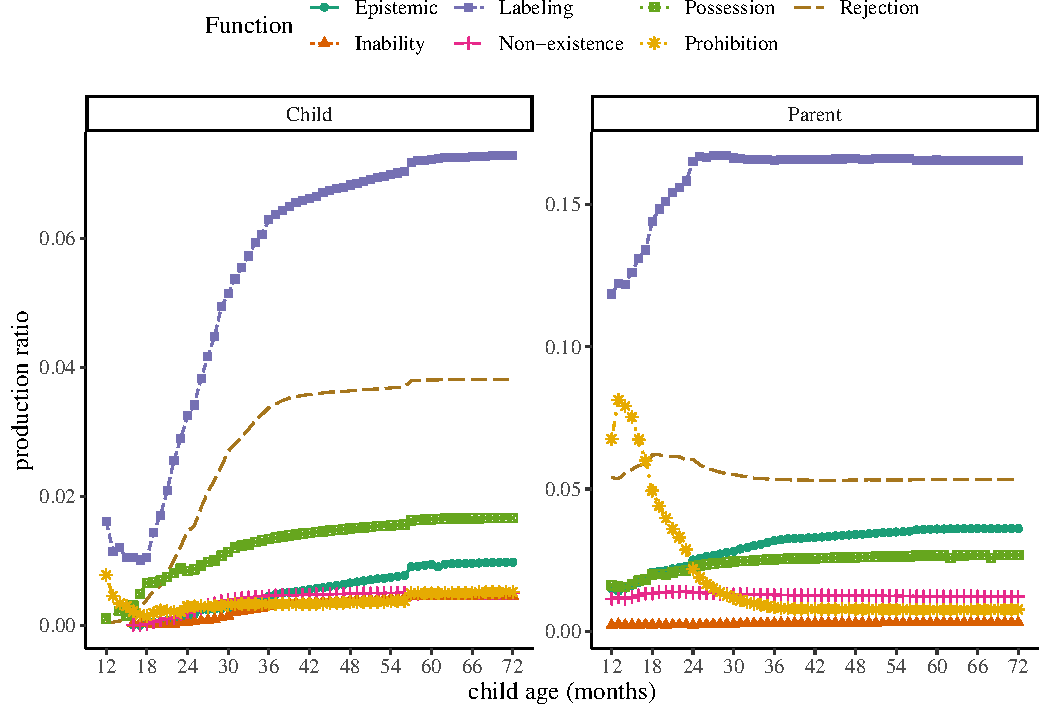
\includegraphics{neg_construction_article_files/figure-latex/allpos-1} 

}

\caption{Cumulative ratios for the positive counpterparts to all negative constructions at the sentence level.}\label{fig:allpos}
\end{figure}

Finally, Figure \ref{fig:alldiscourse} shows the cumulative ratios of all negative responses to a previous utterance that used the negative constructions or their positive counterparts. With parents' production on the right, we see again a relatively constant rate of producing negative responses to each construction after 36 months. Before 36 months, however, most constructions show a gradual increase with the exception of prohibitions. Parents' start with more frequent ``\emph{no!}''-responses to imperatives produced by children, but the frequency of these negative responses drops to a relatively low and stable level after children are 36 months of age; this pattern, again corresponds to parents' production of subjectless imperatives in Figure \ref{fig:allneg} and Figure \ref{fig:allpos}.

\begin{figure}[H]

{\centering 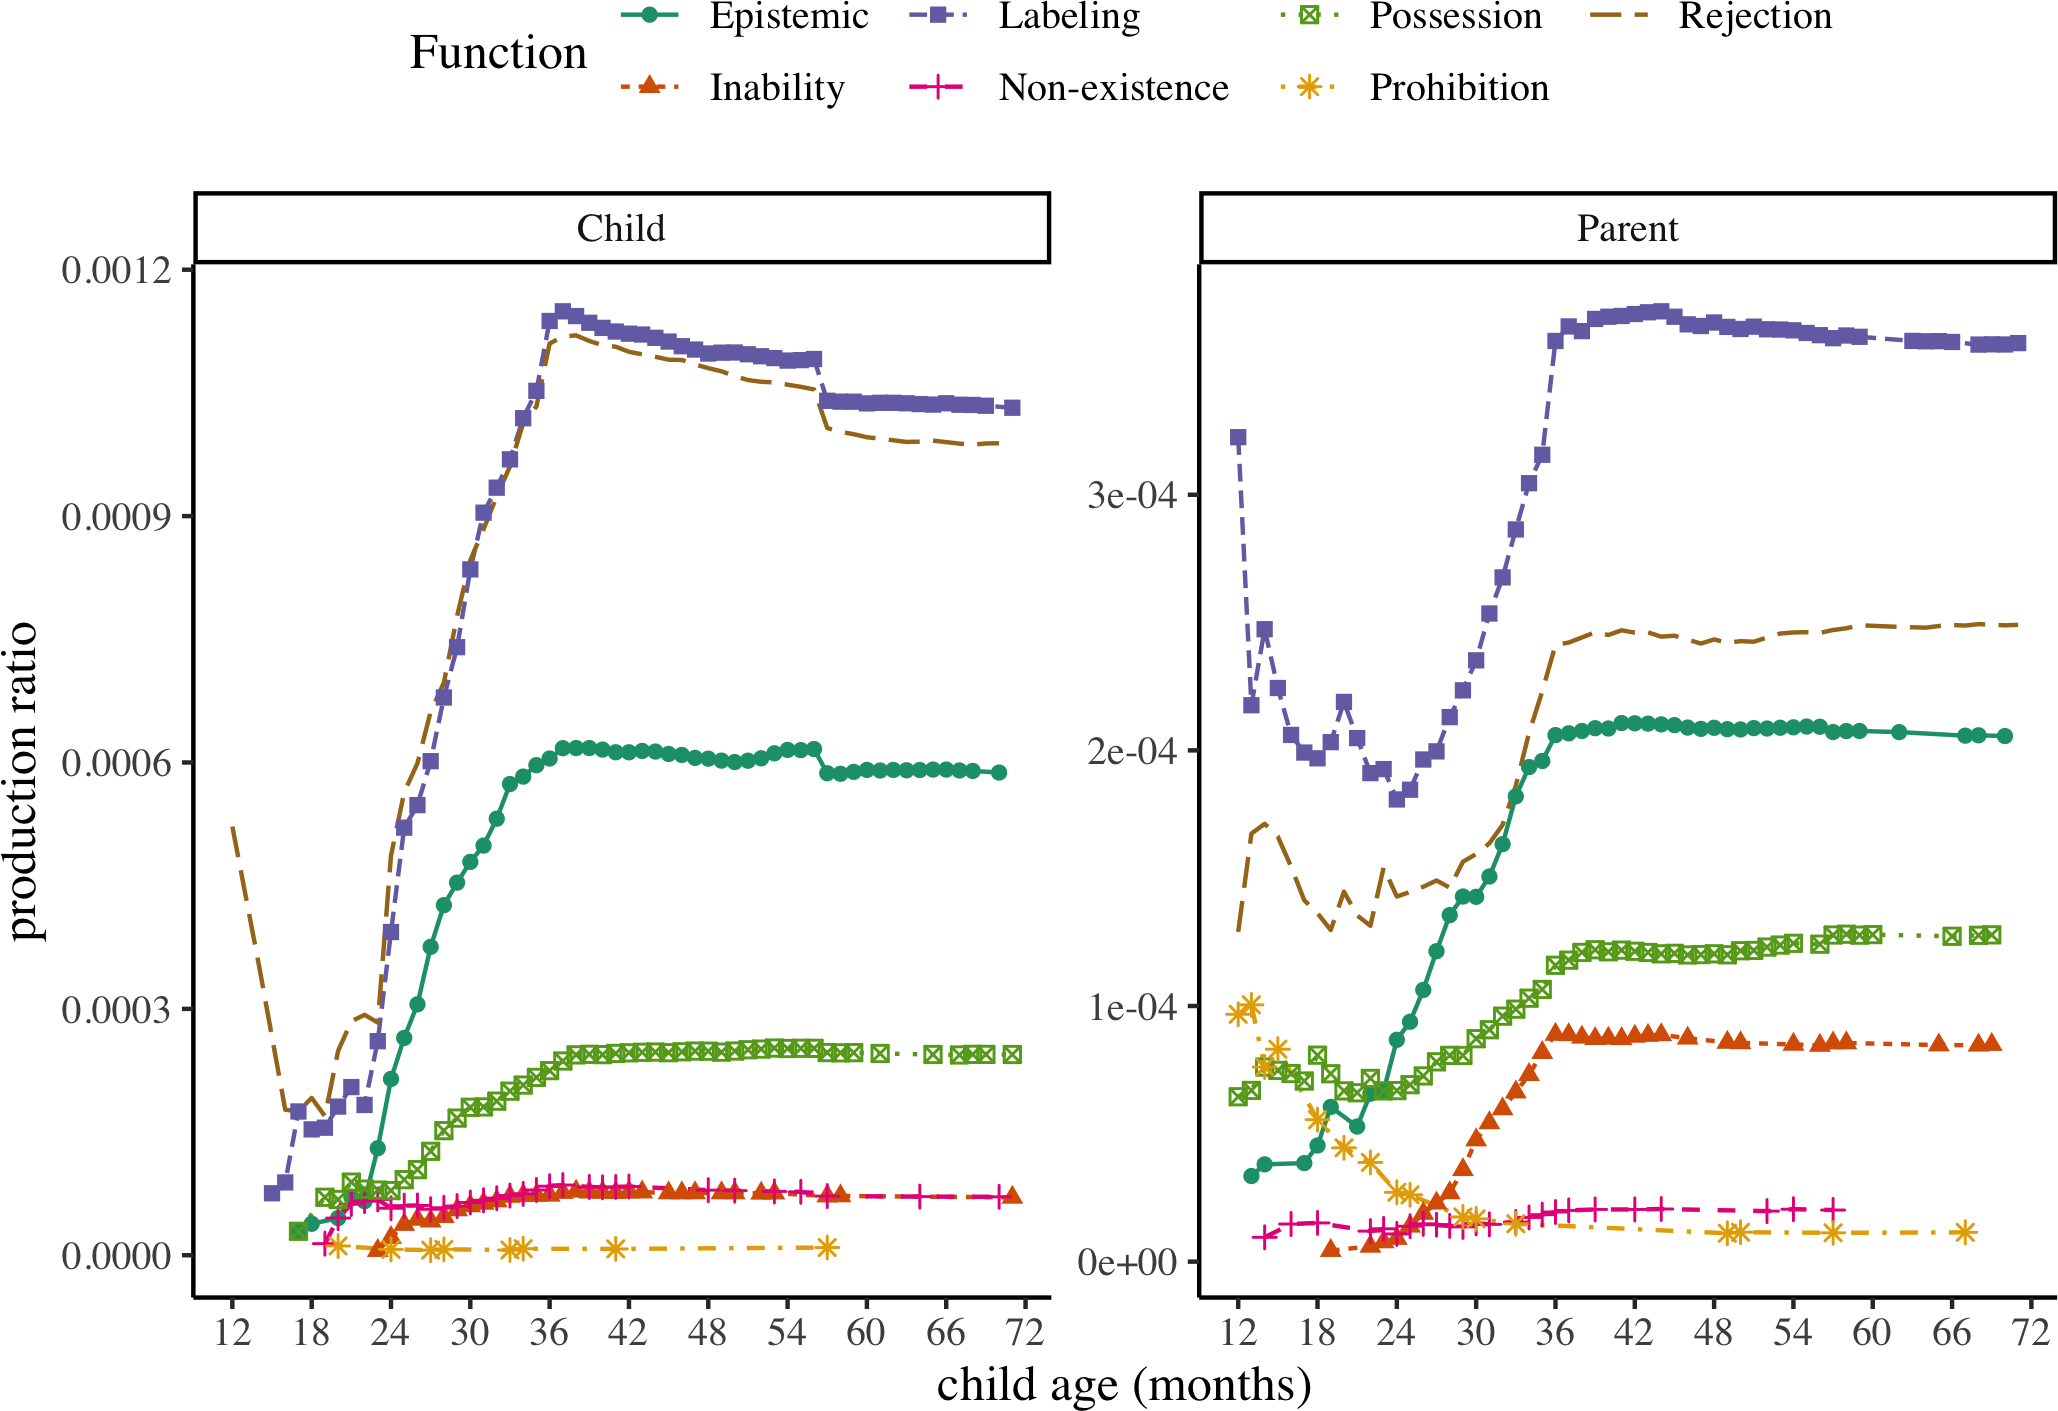
\includegraphics{neg_construction_article_files/figure-latex/alldiscourse-1} 

}

\caption{Cumulative ratios for all negative constructions at the discourse level.}\label{fig:alldiscourse}
\end{figure}

Looking at children's negative responses on the left panel, we see that production begins for most functions around 18 months of age and by 36 months children are also producing negative responses at a relatively constant rate; these patterns draw similarity to those at the sentence level. The comparability of the developmental trajectories for different communicative functions at the discourse level shown in Figure \ref{fig:alldiscourse} is strengthened further with the logistic growth curves. As demonstrated in Table \ref{tab:growthdiscourse}, the asymptotic levels across functions are estimated to be similar to each other; same holds for the maximum growth rate and the age of one-half production growth. Furthermore, the results of the growth curve models at the discourse level are also comparable to those at the sentence level presented in Table \ref{tab:growthsyntax}, indicating overall similar production trajectory between the two levels.

\begin{longtable}[]{@{}
  >{\raggedright\arraybackslash}p{(\columnwidth - 8\tabcolsep) * \real{0.18}}
  >{\raggedright\arraybackslash}p{(\columnwidth - 8\tabcolsep) * \real{0.26}}
  >{\raggedright\arraybackslash}p{(\columnwidth - 8\tabcolsep) * \real{0.18}}
  >{\raggedright\arraybackslash}p{(\columnwidth - 8\tabcolsep) * \real{0.29}}
  >{\raggedright\arraybackslash}p{(\columnwidth - 8\tabcolsep) * \real{0.09}}@{}}
\caption{\label{tab:growthdiscourse} Results for Bayesian logistic growth curve modeling in child speech at the discourse level; 95\% credibal intervals for each parameter were derived from their own postierior distribution.}\tabularnewline
\toprule
Function & Asymptotic level & Growth rate & Age of 1/2 growth & \(R^2\) \\
\midrule
\endfirsthead
\toprule
Function & Asymptotic level & Growth rate & Age of 1/2 growth & \(R^2\) \\
\midrule
\endhead
Rejection & 0.17 (0.02, 0.45) & 0.50 (0.09, 0.90) & 41.95 (39.99, 43.88) & 0.50 \\
Non-existence & 0.22 (0.03, 0.58) & 0.50 (0.09, 0.90) & 41.95 (39.99, 43.91) & 0.50 \\
Prohibition & 0.23 (0.03, 0.59) & 0.50 (0.09, 0.90) & 41.94 (39.94, 43.88) & 0.50 \\
Inability & 0.25 (0.03, 0.66) & 0.50 (0.10, 0.90) & 41.93 (39.92, 43.90) & 0.50 \\
Labeling (Denial) & 0.15 (0.02, 0.42) & 0.50 (0.09, 0.90) & 41.96 (39.99, 43.92) & 0.50 \\
Epistemic & 0.19 (0.02, 0.51) & 0.50 (0.09, 0.91) & 41.94 (39.99, 43.85) & 0.50 \\
Possession & 0.25 (0.03, 0.65) & 0.50 (0.09, 0.91) & 41.94 (39.96, 43.86) & 0.50 \\
\bottomrule
\end{longtable}

\hypertarget{conclusion}{%
\section{Conclusion}\label{conclusion}}

Using automatic annotations of large-scale corpora of child-parent interactions, we presented production trajectories for seven negative constructions that tend to express rejection, non-existence, prohibition, inability, labeling, epistemic states, and possession (Table 1). The results suggest that the production of almost all these negative constructions (except for prohibition) emerges before or around 18 months, and gradually increases within the 18-36 months age range. Their production frequencies slowly become stable and regular after 36 months and relatively comparable to parents' levels of production. These observations hold at both the sentence level (Figure \ref{fig:allneg} and Figure \ref{fig:allpos}) and the discourse level (Figure \ref{fig:alldiscourse}). Our growth curve analyses demonstrate further the similarity in the developmental path of the negative constructions for each of the functions, in partucular with regards to their estimated asymtote level, maximum growth rate, and the age of one-half production growth. These findings suggest that negation possibly starts as a multi-functional concept; in other words, it develops from several communicative functions more or less at the same time. By contrast, our results do not provide clean-cut evidence for previous claims that the different functions of negation emerge and develop at different stages.

For future work, we would like to explore several directions. First, to more thoroughly examine and potentially model the developmental trajectories of negation in child production, certain production-specific factors (e.g., length of utterance, ease of pronunciation) should be taken into account as well in order to paint a more clear picture about the development of negation. Additionally, to avoid as much ambiguity resulted from the automatic parser as possible, we tried to be restrictive when identifying the negative constructions of interest in our study. This means that the structures analyzed here do not include all constructions modified by the three negative morphemes in English, such as instances where the syntactic head is a noun phrase that does not fall under the category of possession (e.g., ``not table''). It would be worthwile for future studies to take upon these cases to investigate more broadly what lexical items negative morphemes co-occur with, and how the lexical diversity of these structures change along the developmental trajectory.

It is important to note that similar to prior studies, our conclusions are limited to negation in children's production. Systematic experiments testing children's comprehension of negative utterances with different communicative functions are necessary to better understand the origins and developmental trajectory of negation.

A different hypothesis is that from the start, negation is an abstract concept that can serve different communicative functions. The main task of the learner is to break the speech stream, detect negative morphemes like \emph{no}, \emph{not}, or \emph{nt'}, and map them to this abstract meaning. She should then learn to use them appropriately in composition with other words to convey the right communicative function in context. There is either no substantial conceptual development for a logical concept such as negation, or this development is complete by the time the process of form-meaning mapping starts. This account predicts that conceptualy speaking, different communicative functions should be learnable and expressable early on and around the same time. Any delays in the comprehension or production of negative constructions and functions must be due to lack of experience with that construction or limitations in children's productive capacity. Therefore, it is possible for communicative functions of negation to not be comprehended or produced in fixed and ordered stages. Children may vary considerably on what constructions or functions they comprehend or produce earlier.

There are a few theoretical and methodological caveats, however. Studies that hypothesize stages in the development of negation almost exclusively study children's productions. Our methods of data collection and analysis may also affect our ability to provide data for or against these hypotheses.

Nevertheless, there seems to be some consensus among researchers that the crucial period for the development of negation is the period between 18 and 30 months of age. Some researchers suggest that by 36 months, children have an abstract concept of negation that is used to convey a variety of communicative functions (Cameron-Faulkner, Lieven, \& Theakston, 2007; McNeill \& McNeill, 1968; Pea, 1978).

Fourth, previous studies have almost exclusively focused on children's production of negation. A tacit assumption is that children's linguistic production provides a straightforward window into their conceptual development. However, children's linguistic comprehension may differ substantially from their production, and these in turn may differ from their conceptual representations. \ldots{} Therefore, developmental patterns

\begingroup
\setlength{\parindent}{-0.5in}
\setlength{\leftskip}{0.5in}

\endgroup

\hypertarget{refs}{}
\begin{CSLReferences}{1}{0}
\leavevmode\hypertarget{ref-diaparser}{}%
Attardi, G., Sartiano, D., \& Yu, Z. (n.d.). DiaParser attentive dependency parser. \emph{Submitted for Publication}.

\leavevmode\hypertarget{ref-bloom1970language}{}%
Bloom, L. M. (1970). \emph{Language development: Form and function in emerging grammars} (PhD thesis). Columbia University.

\leavevmode\hypertarget{ref-Brown1973}{}%
Brown, R. (1973). \emph{A first language, the early stages}. Cambrdige, Mass: Harvard University Press.

\leavevmode\hypertarget{ref-cameron2007part}{}%
Cameron-Faulkner, T., Lieven, E., \& Theakston, A. (2007). What part of no do children not understand? A usage-based account of multiword negation. \emph{Journal of Child Language}, \emph{34}(2), 251.

\leavevmode\hypertarget{ref-choi1988semantic}{}%
Choi, S. (1988). The semantic development of negation: A cross-linguistic longitudinal study. \emph{Journal of Child Language}, \emph{15}(3), 517--531.

\leavevmode\hypertarget{ref-darwin1872expression}{}%
Darwin, C. (1872). \emph{The expression of the emotions in man and animals}. John Murray.

\leavevmode\hypertarget{ref-de1979form}{}%
de Villiers, P. A., \& de Villiers, J. G. (1979). Form and function in the development of sentence negation. \emph{Papers and Reports on Child Language Development}, \emph{17}, 57--64.

\leavevmode\hypertarget{ref-demuth2006word}{}%
Demuth, K., Culbertson, J., \& Alter, J. (2006). Word-minimality, epenthesis and coda licensing in the early acquisition of {E}nglish. \emph{Language and Speech}, \emph{49}(2), 137--173.

\leavevmode\hypertarget{ref-haspelmath1997indefinite}{}%
Haspelmath, M. (1997). \emph{Indefinite pronouns}. Oxford University Press.

\leavevmode\hypertarget{ref-jespersen1917negation}{}%
Jespersen, O. (1917). \emph{Negation in english and other languages} (Vol. 1). AF H{ø}st.

\leavevmode\hypertarget{ref-kemper1995complexity}{}%
Kemper, S., Rice, K., \& Chen, Y.-J. (1995). Complexity metrics and growth curves for measuring grammatical development from five to ten. \emph{First Language}, \emph{15}(44), 151--166.

\leavevmode\hypertarget{ref-macwhinney2000childes}{}%
MacWhinney, B. (2000). \emph{The CHILDES project: Tools for analyzing talk. Transcription format and programs} (Vol. 1). Psychology Press.

\leavevmode\hypertarget{ref-mcneill1968}{}%
McNeill, D., \& McNeill, N. (1968). What does a child mean when he says "no"? In E. M. Zale (Ed.), \emph{Studies of child language development} (pp. 51--62).

\leavevmode\hypertarget{ref-nordmeyer2018individual}{}%
Nordmeyer, A., \& Frank, M. C. (2018). Individual variation in children's early production of negation. In \emph{Proceedings of the 40th annual meeting of the cognitive science society} (pp. 2167--2172).

\leavevmode\hypertarget{ref-pea1978}{}%
Pea, R. (1978). \emph{The development of negation in early child language} (PhD thesis). University of Oxford.

\leavevmode\hypertarget{ref-qi-etal-2020-stanza}{}%
Qi, P., Zhang, Y., Zhang, Y., Bolton, J., \& Manning, C. D. (2020). {S}tanza: A python natural language processing toolkit for many human languages. In \emph{Proceedings of the 58th annual meeting of the association for computational linguistics: System demonstrations} (pp. 101--108). Online: Association for Computational Linguistics. \url{https://doi.org/10.18653/v1/2020.acl-demos.14}

\leavevmode\hypertarget{ref-sanchez2019childes}{}%
Sanchez, A., Meylan, S. C., Braginsky, M., MacDonald, K. E., Yurovsky, D., \& Frank, M. C. (2019). Childes-db: A flexible and reproducible interface to the child language data exchange system. \emph{Behavior Research Methods}, \emph{51}(4), 1928--1941.

\leavevmode\hypertarget{ref-dg}{}%
Tesnière, L. (1959). \emph{{É}l{é}ments de syntaxe structurale}. Paris: Klincksieck.

\leavevmode\hypertarget{ref-wei2006time}{}%
Wei, W. W. (2006). Time series analysis. In \emph{The oxford handbook of quantitative methods in psychology: Vol. 2}.

\end{CSLReferences}


\end{document}
